%
% TU/e Style Master Thesis template for LaTeX
%
% Public version 1.0
% 2010 - 2013 Thijs Nugteren and Joos Buijs
%
% THIS IS THE MAIN FILE (i.e. compile this file, compiling the others directly won't work)
%
\documentclass[a4paper,10pt,twoside]{report}

%all the other includes etc. are done in the thesis.sty file.
\usepackage{thesis}

%
% These commands need to be defined in order to produce a correct and personalized document
%
\newcommand{\shortdoctitle}{Master's Thesis}
\newcommand{\doctitle}{Efficient Graph Processing Using AWS S3}
\newcommand{\docsubtitle}{Master Thesis}

\newcommand{\me}{Aditya Chandla}
\newcommand{\keywords}{Graph Databases, Serverless}
\newcommand{\version}{1.0}
\newcommand{\monthYear}{July 2024}

%Be sure to use all the titles for your committee members!!! (their names show up on the very first page!)
\newcommand{\firstCommitteeMember}{dr. Nikolay Yakovets}
%\newcommand{\secondCommitteeMember}{Your second Committee Member, usually the daily supervisor}
%\newcommand{\thirdCommitteeMember}{Your Third Committee Member, usually the external member}

\author{\me}

%
% PDF settings
%
\hypersetup
{
    pdfauthor={\me},
    pdftitle={\shortdoctitle},
    pdfsubject={\doctitle},
    pdfkeywords={\keywords}
}

\begin{document}

%use this include for PDF and distribution versions
\pagenumbering{roman}
\begin{titlepage}
\begin{center}

\includegraphics[height=2cm]{figures/tue-logo-high}\\
%\LARGE
%Eindhoven University of Technology \\
\large
Department of Mathematics and Computer Science  \\
Database Group

\vspace*{10cm}

\setlength{\TPHorizModule}{1mm}
\setlength{\TPVertModule}{\TPHorizModule}
% Set the Paragraph Indent to zero, so the first line is not Indented
% Back-up the current value so it can be put back at the end of the title page
\newlength{\backupparindent}
\setlength{\backupparindent}{\parindent}
\setlength{\parindent}{0mm}			
% Begins a textbox at 72 mm from the left of the edge of the paper and 89 mm from the top
% The width of the textbox is 95 mm (167 - 72 mm)
% The height of the box cannot be defined, so it is your task to keep the text not too long
\begin{textblock}{95}(62,89)
    \vspace*{1mm}
    \huge
    \textbf{\doctitle \\}
    \Large
    \vspace*{5mm}
    \textit{\docsubtitle}\\
    \vspace*{10mm}
    \Large
    \me\\
\end{textblock}

\large
Supervisors:\\
\begin{tabular}{rl}
    \firstCommitteeMember\\
    \secondCommitteeMember\\
    \thirdCommitteeMember\\
\end{tabular}

%\vfill
%\version

\vfill
%\docdate \\
\large
Eindhoven, \monthYear\\

% Put the Paragraph Indent back to its original value
\setlength{\parindent}{\backupparindent}
\end{center}
\end{titlepage} 


\normalsize

\clearemptydoublepage

%Sometimes line numbers are nice, uncomment the next line to enable:
%\linenumbers

%It could be handy to have a list of todos and brainstorms in your thesis
%\chapter*{*General todos*}\todo{remove this chapter}
%\input{chapters/general_todos}

%\chapter*{*Brainstorm results*}\todo{remove this chapter}
%\input{chapters/brainstorm_results}

\chapter*{Abstract}\label{chapter:abstract}
As the size of graphs being queried by graph databases increases, coupling 
storage and compute increases the cost and limits the flexibility of
traditional graph database management systems (GDBMS). As part of this thesis,
we explore the viability of an architecture where the compute and storage are
independent. This independence is achieved using a distributed cloud storage
service (AWS S3) which provides bottomless storage and theoretically unlimited
throughput. Using this distributed cloud storage solution, we evaluate the
latency of running two common graph traversal algorithms i.e breadth first
search (BFS) and depth first search (DFS). We then compare this latency with
some other systems which may be used to perform BFS and DFS on large graphs.
Lastly, we also provide a cost model to evaluate the cost effectiveness of our
approach for various use cases.


\clearemptydoublepage

%An executive summary if you want:
%\chapter*{Executive summary}\label{chapter:executive_summary}
%\input{chapters/executive_summary}

%\clearemptydoublepage


\chapter*{Preface}\label{chapter:preface}
This thesis was completed as part of the Master of Computer Science
program at TU Eindhoven. This specific project was carried out within the
Databases group and under the guidance of dr Nikolay Yakovets. First and
foremost, I would like to thank Nick for letting me decide the topic and
contents of this project. This gave me experience with how to go from a
vague idea to concrete research questions. Successfully navigating this process gave me
confidence in my ability to explore the research on a particular topic and
discover research gaps. Nick's guidance was also crucial in keeping the project
on course, preventing me from getting bogged down in trivialities. Furthermore, 
his insights often revealed interesting
questions that I had not originally planned to explore but incorporating those
insights has enhanced the comprehensiveness of this work and, hopefully, the
reading experience. I would also like to thank my friends and colleagues who have
made my life outside academics more enjoyable. Finally, I would like to thank my
parents for enabling for me to study at TU Eindhoven and for providing
constant support and encouragement throughout my degree.



\clearemptydoublepage

\tableofcontents

\clearemptydoublepage

\listoffigures

\clearemptydoublepage

\listoftables

\clearemptydoublepage

\lstlistoflistings

\clearemptydoublepage

\chapter{Introduction}\label{chapter:introduction}
\setcounter{page}{0}
\pagenumbering{arabic}
%from here on, start the 'real' page numbering, from 1, with normal digits
In a recent survey titled `Ubiquity of large graphs'\cite{sahu2017ubiquity}, the
authors noted that the size of graphs being used in both academia and industry
is increasing. Although this survey found that it was common for graphs to have
tens of billions of edges, it also found that scalability was the primary
concern of all the participants surveyed\cite{sahu2017ubiquity}. In this thesis,
we evaluate one way to alleviate this concern of scalability by decoupling
storage of base graph from the query evaluation.

\medskip
Today, all major cloud providers have a distributed cloud storage offering,
Google cloud platform offers Google cloud storage\cite{gcpStorage}, Azure offers
Azure Blob storage\cite{azureStorage}, and AWS offers Simple Storage Service or 
S3\cite{awsS3}. These distributed storage services are already used by Big Data
Analytics tools like Snowflake\cite{snowflake} and RDBMSs like Neon\cite{neonPostgres} 
for storage of underlying data. The use of these distributed storage services has not
yet been explored for storing and querying graph data.

\section{Research Question}
In this paper, we provide an initial analysis of how distributed storage services can 
be used to query large graphs. While using these distributed storage services, the primary
issue that needs to be addressed is of latency. The latency of accessing data in a networked
distributed system involves communication over the network which is at least three orders of
magnitude more than accessing data from local storage. In return for this increased latency,
we get virtually unlimited throughput as read operations are distributed across a cluster 
of thousands of physical machines if not more. Therefore, in this paper, we evaluate ways to
reduce the latency of accessing graphs. We will focus on the 
performance of two commonly used graph traversal algorithms: Breadth first search 
(BFS) and Depth first search (DFS). More formally, the first research
objective is as follows:
\begin{displayquote}
    \textbf{RO 1:} Gauge the effectiveness of caching and prefetching techniques
    on the latency of graph access for graph traversals.
\end{displayquote}

\medskip
Apart from reducing the latency, we will also discuss how the cost model of
distributed storage engines is different from the traditional model of coupled
compute and storage. For storage engines like S3, we are charged for every
gigabyte of storage and we are charged for every request that we make on that
storage. On the other hand, in case of an SSD/HDD storage unit, you pay for a
certain amount of storage and there is no additional cost for accessing the
storage. Therefore, we seek to provide a model to help users choose between one
form of storage over the other. More formally, the second research objective is
as follows:
\begin{displayquote}
    \textbf{RO 2:} Provide a cost model to help users decide whether using S3
    instead of SSD/HDDs might be more cost effective.
\end{displayquote}


\section{Structure of the thesis}

\medskip
In Chapter-\ref{chapter:preliminaries}, we provide the necessary background for
this thesis. In Section-\ref{sec:distributedStorage} we talk about the
history, architecture, and characteristics of distributed storage systems. We
also give a brief overview of the capabilities of AWS S3, which is the service
that we use in this thesis. Then,
in Section-\ref{sec:serverlessArch}, we discuss the advantages of database
architecutres which separate compute and storage. Finally, in
Section-\ref{sec:cachingDistSys} we discuss the caching and prefetching
strategies that we employ in this thesis to lower the latency of graph
traversals.

\medskip
In Chapter-\ref{chapter:systemArchitecture}, we introduce our architecture for
performing traversals. We start by providing a description of each component and their
responsibilities in Section-\ref{sec:componentOverview}. After that, we describe
the traversal queries which will be evaluated by our system in Section-\ref{sec:queryEvaluation}.
Then we provide a baseline implementation which we will be useful for comparing
the impact of the improvements made in the subsequent sections. Finally, in
Sections-\ref{sec:graphAccess}, \ref{sec:parallelAlgorithms}, and
\ref{sec:partitionSize}, we describe the details of our proposed architecture
which enables low latency traversals for large graphs.

\medskip
In Chapter-\ref{chapter:evaluation}, we present the results of the
implementation of the proposed system architecture. We begin this chapter by
comparing the performance with the baseline solution in
Section-\ref{sec:cmpBaseline}. Then in Section-\ref{sec:cmpOtherTools}, we
compare the performance of our solution with Neo4j and Apache Flink. This
section highlights various characteristics of different types of tools(GDBMS,
RDBMS, Big Data tools, and Custom Solutions) and the areas in which they 
are suitable. 

\medskip
In Chapter-\ref{chapter:discussion}, we elucidate the reasoning for various choices
made throughout the thesis.
In Section-\ref{sec:altArchitectures} we discuss other possible architectures for
performing traversals on large graphs using S3 and their advantages and
disadvantages over the proposed architecture. Then, in
Section-\ref{sec:useCases}, we discuss the use cases where this architecture
can be more cost efficient and flexible compared to other tools and where users
would be better off avoiding this architecture. Finally, in
Section-\ref{sec:threats}, we consider the threats to the credibility of this
work.

\medskip
Finally, in Chapter-\ref{chapter:conclusions}, we conclude the thesis and
suggest possible directions for future work. This section contains information
about how we may be able to extend this work to reach a point where we have a
fully functioning graph database whose storage resides in S3.


\clearemptydoublepage

\chapter{Preliminaries}\label{chapter:preliminaries}
The purpose of this thesis is to reduce the latency of graph access in cases
where the graph is stored on a distributed file system like AWS S3. To
put this work into context, we start by providing an overview of distributed
storage services and more details about the particular storage service that
will be used in this thesis. Then, we provide background on the idea of
separating compute and storage, the evolution of this idea, and its
applicability. After that, we describe the current literature on how others have
approached the idea of reducing access latency by using caching algorithms. We
end this section by comparing the contributions of this research with the
current state-of-the-art in the field of graph databases.

\section{Distributed storage services}\label{sec:distributedStorage}
The idea of accessing files via the network can be traced back to the early days
of the internet. However, the first widely used implementation of a networked
file system was developed by SUN Microsystems\cite{nfs1986}. Their implementation
is widely referred to as the networked file system (NFS). Their implementation
provided users with the ability to mount a file system present on a remote
machine. However, this system did not provide any distribution transparency, as
the users had to be aware of where and how each file was stored on remote
machines. 

\medskip
The first widely used implementation of a distributed file system is considered
to be the Hadoop Distributed File system (HDFS)\cite{shvachko2010hadoop}. This
implementation provided distribution transparency and consistency guarantees on
various operations on the files stored in HDFS. This implementation was inspired
by the Google File-system\cite{ghemawat2003google}, which was developed by Google
almost seven years before HDFS.

\medskip
Although systems like HDFS were widely used, distributed file systems like AWS
S3\cite{awsS3} provided an additional feature of being multi-tenant. In other
words, with file systems like AWS S3, a user could reap the benefits of a
distributed file system without having to manage or pay for an entire cluster.
The cost of managing, scaling, and maintaining the distributed cluster was
delegated to cloud providers like AWS. Now, users could pay for the amount of
data that they store, and the number of requests that they make to their data.
This has enabled the usage of such distributed file systems in applications like
video streaming, database storage\cite{snowflake}, web content 
delivery, and backup storage.

\begin{figure}[ht]
    \centering
    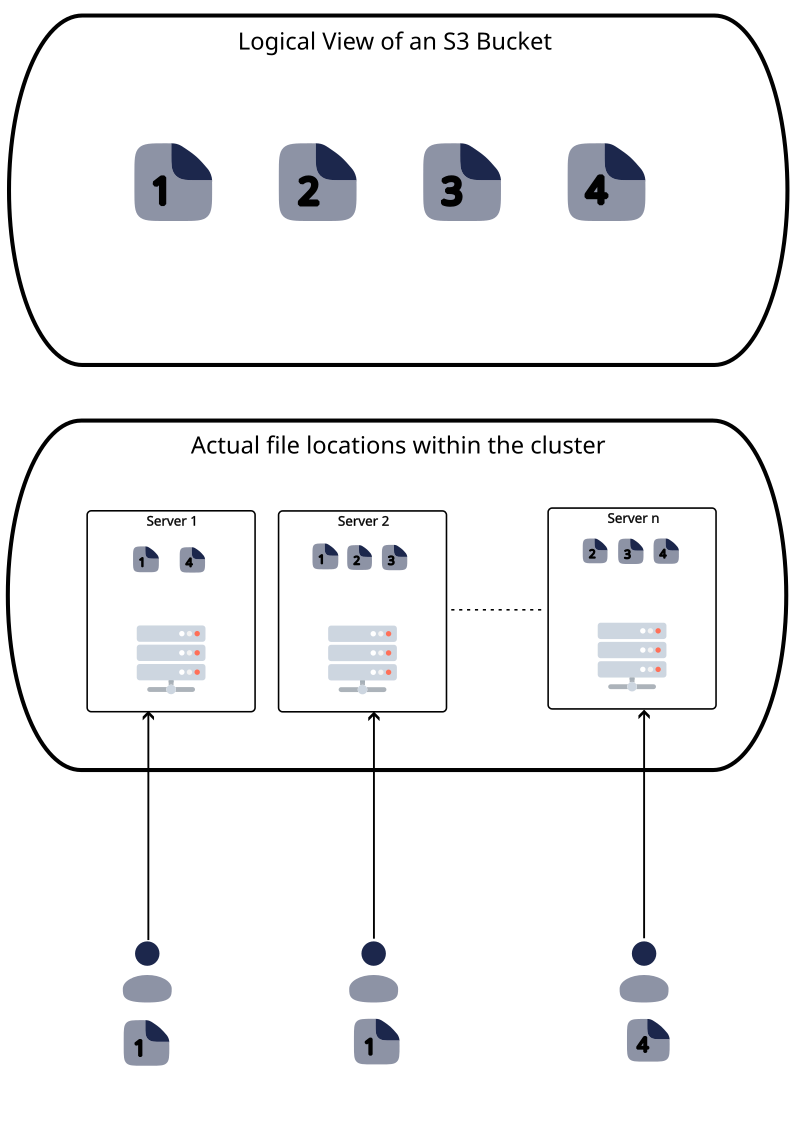
\includegraphics[width=0.65\textwidth]{figures/distributedCloudStorage.png}
    \caption{Distributed File Store}
    \label{fig:distFileStore}
\end{figure}

\medskip
The exact architecture of AWS S3 or any similar service provided by
competing cloud providers is not known precisely. However, we can glean some information
about S3 based on
how other distributed file systems were designed. We will explain some basic ideas
related to AWS S3 using Figure-\ref{fig:distFileStore}. Let us assume we need to
store four files in AWS S3. To do that, we first create a storage unit
called a `bucket', which is similar to a directory in a file system. After
uploading our files to this bucket, the files get replicated over the entire AWS S3 cluster in
that particular region. Figure-\ref{fig:distFileStore} assumes that this cluster
has a replication factor of two, and therefore, every file is stored on two
physical servers. Now, if users send requests to access these files, their
requests can be redirected to any one of the servers containing the desired file. For
example, if the first and the second user both want to access file number 1, their
requests can be served by two different servers since the same copy will be
saved on two different servers. For simplicity, the figure shows that users make
direct requests to the physical machines containing these files. However, in
reality, they all send requests to a single endpoint, and their requests are then
redirected to a server based on some load-balancing scheme. In later chapters,
we will use this abstract model of a distributed file system to argue about the
applicability of various techniques.

\medskip
Apart from the basic understanding of AWS S3 as it relates to a distributed
file system, we also want to draw the reader's attention to the following
characteristics of AWS S3 as mentioned in its documentation:
\begin{enumerate}
    \item \textbf{Throughput SLA}: At the time of writing this paper, AWS
        guarantees that S3 can handle at least 5500 requests per object stored
        in a bucket. Note that there is no restriction on the total number of
        objects that can be stored in a bucket.
    \item \textbf{Storage Classes}: S3 offers various storage classes that have
        different cost and performance characteristics. These storage classes
        determine how much you pay for storage and for making requests. In this
        thesis, we make use of the `S3 Standard' and `Express One Zone' storage
        classes.
    \item \textbf{Costs}: The cost of using AWS S3 depends on two factors: total
        storage and number of requests. The storage cost for `S3 Standard'
        storage class is \$0.023/GB and the cost of GET requests is
        \$0.0004/1k requests. However, the storage cost for the lower latency
        `Express One Zone' storage type is higher with \$0.16/GB, but the cost of making
        requests is lower at \$0.0002/1k requests. 
    \item \textbf{Artificial sub-directories}: Although AWS CLI and other tools
        provide the capability to upload and navigate a bucket like a directory,
        the underlying architecture only supports having files inside a
        bucket. Therefore, if you have a folder `f1' with two files `one' and
        `two', unlike a file system, the bucket would only contain two files:
        `f1/one' and `f1/two'. The name of the folder is
        prepended to the file names.
    \item \textbf{Hashing object names}: To decide which partitions an
        object is assigned to, S3 internally hashes the first few characters of
        the filename. Therefore, if we have object names whose first few
        characters are the same, they may all be assigned to a
        single partition, which may lead to lower performance. Although it is
        known that S3 automatically splits partitions in case of overload,
        there is some overhead and time delay in performing the split.
    \item \textbf{Consistency}: Despite being a distributed system, AWS S3
        provides a strong `Read-After-Write' consistency. This means that any
        updates to an object are immediately visible to all clients.
\end{enumerate}

\section{Separating compute and storage}\label{sec:serverlessArch}
One of the first proposed implementations of a database with separate compute and
storage can be traced back to 2008\cite{brantner2008building}, where Brantner et
al. proposed an architecture of a relational database that used AWS S3 as its
storage layer. The authors of this paper primarily focused on how to handle
updates under various consistency models when the data is stored in S3. This
idea was further developed over the years by AWS and culminated with the release
of AWS Aurora\cite{verbitski2017amazon}. Although Aurora separated compute and
storage, the write throughput was still limited because all write
traffic was directed to a single instance. The first database to support
multiple read and write instances on top of distributed data is considered to be
Snowflake\cite{dageville2016snowflake}. Their architecture was built upon the
storage layer of AWS S3. On top of this storage layer, users could create as many `virtual
warehouses' as they needed. Since then, various databases with independent
storage and compute planes like Neon\cite{neonPostgres} and AWS Aurora
Serverless\cite{auroraServerless} have been released.

\medskip
The term `Serverless databases' is often used for databases with separate
compute and storage; however, these two concepts are different. A `serverless
database' has a pay-as-you-go model where you pay for the amount of storage that
your databases use, and the compute resources that were used in a fixed amount
of time. In this model, the users simply have to define the minimum and maximum
compute resources that the database can use and the database scales according
to the load. Note that the definition of serverless database does not
necessitate separation between compute and storage, and there are indeed
databases like CockroachDB\cite{taft2020cockroachdb} which offer a serverless
model although the underlying architecture couples storage and compute together.
Therefore, although separating compute and storage may be amenable to a
serverless design, it is not a requirement for it. The term serverless,
therefore, defines a type of payment model, whereas having separate storage and
compute for a database is more of a system architecture choice. 

\medskip
A database that separates compute and storage offers better scalability,
elasticity, and modularity. When the compute and storage are
separated, both of them can be scaled independently. A heavily used service
that has a relatively low amount of data can scale the database's compute without
wasting any storage. On the other hand, a service that has a lot of data but
has a low query workload can scale the database's storage without wasting any
compute. Furthermore, this separation also provides more elasticity so that the
database can seamlessly scale up when the workload increases and can scale down
during low-traffic hours. Finally, separating storage and compute can lead to
more modularity since the storage layer and the compute layer can be upgraded
and changed based on the system's requirements. For example, if a cloud provider
launches a new instance type that is better suited for your workload, you can
switch to the newer instance type without being concerned about data migration.
These aforementioned characteristics make databases with separate compute and
storage attractive to a variety of use cases.

\medskip
Separating compute and storage in databases often comes at the cost of increased
latency. This latency is a result of the network communication between the
storage layer and compute layer that needs to take place to complete any
database operation. Although the throughput of networks has massively increased
in the past few years (AWS offers instances with up to 200 Gbps bandwidth), the
latency of network communication is limited by the speed of light. Therefore, a
database with a local SSD containing all the base data will always be faster
than a database whose storage needs to be accessed over a network. The actual
difference between performance depends on the physical distance between storage
and compute nodes. If the entire deployment is in a single data center, the
latency is around 500$\mu$s, which is still an order of magnitude higher than access latency
for an SSD\cite{jiang2021fusionraid}. This advantage becomes less pronounced in
distributed databases with coupled storage and compute since they may also require
some communication between instances to respond to user queries.
Although there are various caching and prefetching mechanisms to reduce latency
for databases with separate storage and compute, there remain cases where
coupling storage and compute yields lower latencies.


\section{Caching and Prefetching}\label{sec:cachingDistSys}
The concept of caching and prefetching in the case of graphs enables us to take
advantage of spatial and temporal locality to reduce the latency of future graph
accesses. The terms spatial and temporal locality come from literature on
processor caches. In the context of a processor cache, temporal locality refers
to the tendency of a memory location that is accessed now to be
accessed again soon. Similarly, spatial locality refers to the 
tendency of a memory location close to a recently accessed memory location to be
accessed in the near future. These concepts can be translated to graphs as
follows:
\begin{enumerate}
    \item \textbf{Spatial Locality} in case of graphs means that if a node is
        accessed, then it is likely that this node's neighbors will be accessed
        in the near future.
    \item \textbf{Temporal Locality} in case of graphs refers to the existence
        of central nodes according to some centrality metric. There are
        various centrality measures\cite{klein2010centrality}, which may help us 
        identify nodes that are central for a particular graph algorithm. The
        main idea is that there exist some nodes that have a higher probability
        of being accessed while running a particular algorithm on a graph.
\end{enumerate}
In this section, we will discuss some background research on caching and
prefetching, which would help us exploit  spatial and temporal locality to lower
the data access latency for graph traversals.

\medskip
Any caching scheme consists of two fundamental operations: admission of
data to the cache and eviction of data from the cache. There are various cache
eviction policies like Least Recently Used (LRU), Least Frequently Used (LFU)
that define what data to evict from the cache when it becomes
full. There also exist eviction policies that rely on metadata related to the
data to choose the data elements to evict. Such metadata might
include the size of the data element, time of last data access, and access latency
of the element in case of a cache miss. Apart from eviction, a cache also needs
an admission policy, which, in the case of most caches, is to add the data that
caused a cache miss. However, there do exist more sophisticated
admission algorithms like TinyLFU\cite{einziger2017tinylfu}, which make the
admission decision based on metadata related to a data object, which in the case of
TinyLFU is the access frequency of a data item. Storing metadata of an
object often increases memory consumption and maintenance overhead. These
admission and eviction policies determine the effectiveness of a cache algorithm
for a given use case.

\medskip
We will first consider schemes that do not require additional information about
the stored data, like size or access latency, in case of a cache miss. In
this case, LRU and LFU are two of the most commonly used algorithms. It has been
shown that if the access pattern follows Zipf's law\cite{zipf1929relative}, then
LFU outperforms LRU. However, if the access pattern has a high temporal locality,
then LRU can outperform LFU. Therefore, the choice between LRU and LFU depends
on the underlying access pattern of the data. This choice, however, does not
have to be binary as we can also have an LRFU cache\cite{lee2001lrfu}, which
provides us with a way to have an eviction policy that takes both recency and
frequency into account for eviction. This algorithm subsumes both LRU and LFU
because its functioning depends on a factor $\lambda$, which dictates the
weight that is given to recency versus frequency while evicting an item. As a
result, we can tune this parameter to have the cache behave like LRU or LFU.
Thus, with the LRFU cache, we can fine-tune our eviction policy when we do not
have additional information about the items.

\medskip
In the last paragraph, we talked about caching policies when we do not have any
additional information about the stored items; however, while processing
graphs, we do have some information about the graph topology when we access a
node's neighbors. This information can be useful if a node's neighbors are
likely to be accessed. This idea of graph-aware
caching algorithms was introduced by Aksu et al. in a paper where they
introduced a graph-aware caching policy named Clock-based graph-aware
caching (CBGA)\cite{aksu2015graph}. Although the algorithm contains many 
important contributions, the
main idea of this algorithm is to expect that a node's neighbors will be
accessed if a node is accessed. This idea helped their algorithm outperform all
other competing cache algorithms, which did not exploit the structure of the
graph. Their idea was further extended by Bok et al.\cite{bok2020memory}, where
they added a used-cache in addition to a prefetcher cache for speeding up
sub-graph lookups. This idea helped them outperform CBGA for the task of sub-graph
matching where they achieved a hit ratio of between 50\% and 65\%. 
These contributions highlight the potential for graph-aware caching to
reduce the latency of graph access.

\section{Comparison with State-of-the-Art}\label{sec:cmpSOTA}
In the field of graph databases, there are two types of databases based on how
they store the underlying graph data: native graph databases and non-native graph
databases. Native graph databases (like Neo4j\cite{neo4j}) use data structures that are 
optimized for
graph traversals and thus, usually deliver better performance for graph
navigation operations. Non-native graph databases (like Amazon Neptune\cite{neptune}) rely 
on storage mechanisms of
relational databases, key-value stores, or document stores to store the
underlying graph. In this paper, we propose an architecture that leverages
distributed storage services to store graphs in a native graph data structure. 


\smallskip
This architecture is a unique contribution because most native graph databases 
couple storage and compute together. Graph databases like Neo4j and
Memgraph\cite{memgraph} require all the
data to be present on a single machine. Although Neo4j supports sharding of
graph data, the onus of doing so is primarily put on the user. There are some
closed-source databases like Tigergraph\cite{tigergraph} that support automatic sharding, 
but the storage and compute are tied together. In this landscape of graph 
databases, we aim to explore the
viability of a graph storage architecture that leverages distributed storage
systems. In this architecture, all the graph data would be present on the
distributed file system, and queries on this data would be served by stateless
compute instances. This separation would provide bottomless storage and the
ability to scale up or scale down compute easily. This ability to deliver
practically infinite storage and compute elasticity is a feature missing from
most native graph databases. Later in this thesis, we compare the performance (Section
\ref{sec:cmpOtherTools}) and the cost (Section \ref{sec:costModel}) of our architecture with
other tools that may be used for traversing graphs.


\clearemptydoublepage

\chapter{System Architecture}\label{chapter:systemArchitecture}
\section{Component Overview}\label{sec:componentOverview}
Figure \ref{fig:sysArch} contains the high-level overview of the system that
we will use for query evaluation. We will now give a brief explanation of the
components present in this figure:
\begin{enumerate}
    \item \textbf{LDBC}: The Linked Data Benchmark Council(LDBC) publishes datasets
        for various types of graph processing workloads. In this thesis, we make
        use of the Social Network Benchmark (SNB) datasets in order to evaluate
        the performance of our traversals.
    \item \textbf{LDBC Converter}: The LDBC dataset are in CSV format and
        contain additional information about nodes and edges. As we will explain
        in Section \ref{sec:modifiedCsr}, we need the data to be in a particular
        binary format and we do not have any use for node and edge properties.
        This component of the system removes the unnecessary information from
        the LDBC datasets and maps the data into the desired binary format.
    \item \textbf{AWS S3}: Once the LDBC converter converts the data into a
        binary format, this data is added to an AWS S3 bucket. A `bucket' in AWS S3
        is a container for files.
    \item \textbf{Graph Access Service}: This service provides an interface for
        accessing a graph stored in AWS S3. This interface provides its users
        the ability to get a node's neighbours by providing
        the source node, edge label, and edge direction. This service contains
        all the caching mechanisms that we will use to reduce the latency of
        traversals. We will discuss this service in more detail in
        Section \ref{sec:graphAccess}.
    \item \textbf{Graph Algorithm Service}: This service is responsible for
        using the interface provided by the graph access service to perform
        traversals and measure their performance. We discuss this component in
        more detail in Section \ref{sec:parallelAlgorithms}.
\end{enumerate}
\begin{figure}[ht]
    \centering
    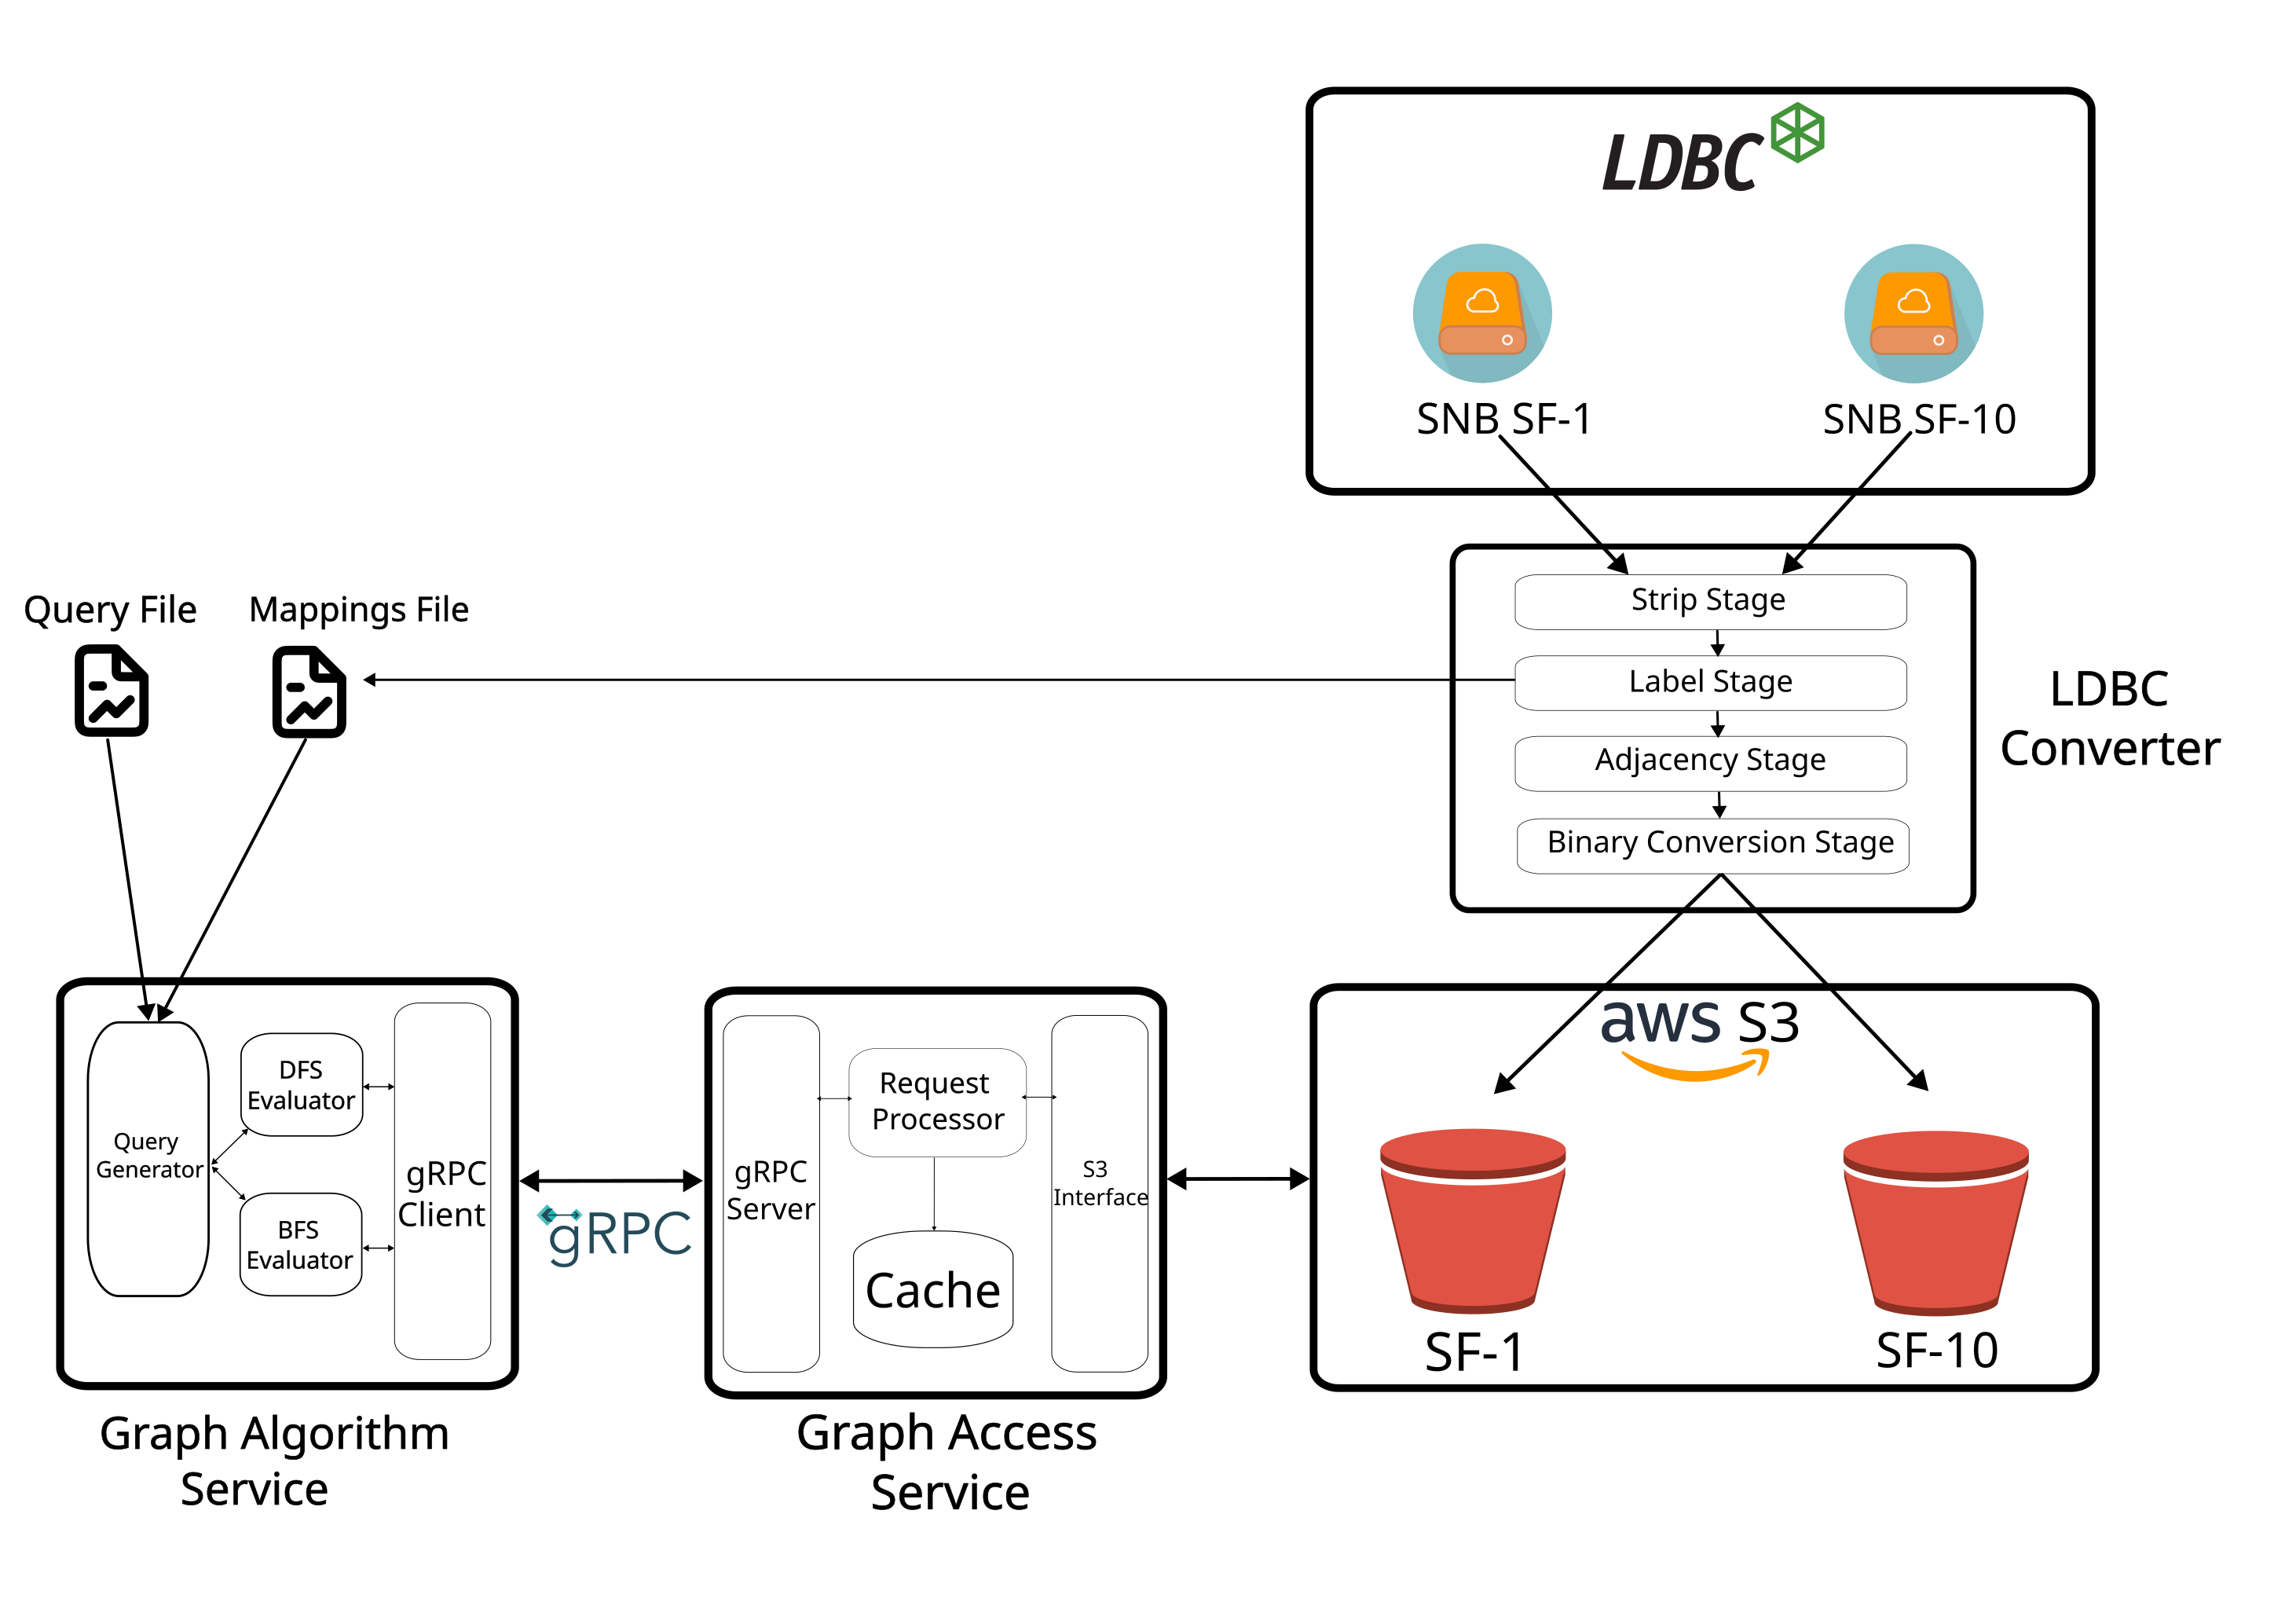
\includegraphics[width=0.9\textwidth]{figures/architecture.png}
    \caption{High Level System Architecture}
    \label{fig:sysArch}
\end{figure}

Looking at the architecture in Figure \ref{fig:sysArch}, it is natural to wonder
why we have two separate services for accessing the graph and performing
traversals on that graph. There are two reasons for this separation: first, it
separates the logic for accessing graphs from the logic for performing
traversals with minimal overhead; second, this type of architecture is
particularly amenable to creation of a multi-tenant storage layer, as used
in the Neon database \cite{neonPostgres}. This is why we have chosen to separate
the service responsible for accessing the graph and caching from the service
responsible for running traversal algorithms.

\section{Baseline Implementation}\label{sec:baseline}
Since there are no existing tools that we can use to compare our solution with,
we present a baseline implementation to gauge the effectiveness of our caching
techniques and algorithmic improvements that we will present in the following
sections. The main idea of the baseline implementation is to provide the most
straightforward way to perform traversals on a graph that is stored in AWS S3.

\medskip
As per the workflow we presented in Section \ref{sec:componentOverview}, we
first need to convert the graph from the LDBC dataset into a format that
enables us to fetch parts of the graph that we need for processing. In order to
do this, we convert the graph into an adjacency list, then we partition that
adjacency list based on size, and finally convert it to compressed sparse
row (CSR) format \cite{duff1984computer}. With this partitioned CSR format stored
in AWS S3, our aim is to load the desired file whenever we want to fetch a node's
neighbours.

\medskip
Figure \ref{fig:baselineImpl} shows the design of graph access service and graph
algorithm service for this baseline implementation. The graph algorithm service,
is responsible for performing the traversals and recording the results. This
service uses the textbook implementation of DFS and BFS, with the only caveat
that a node's neighbours are requested from the graph access service. The graph
access service contains an index which maps node ranges to AWS S3's file names. With
this index, we can get the file name for the AWS S3 file which contains a particular
node's neighbours. Additionally, this service also contains an LRU cache of some
files that were fetched from AWS S3. The size of this cache is limited because each
cache entry contains an entire file with adjacency information for
hundreds of nodes. With these components in place, whenever the graph access
service gets a request, it first checks if that request can be served from the
cache; if not, we fetch the file corresponding to the requested node and add
that file to the cache.
\begin{figure}[ht]
    \centering
    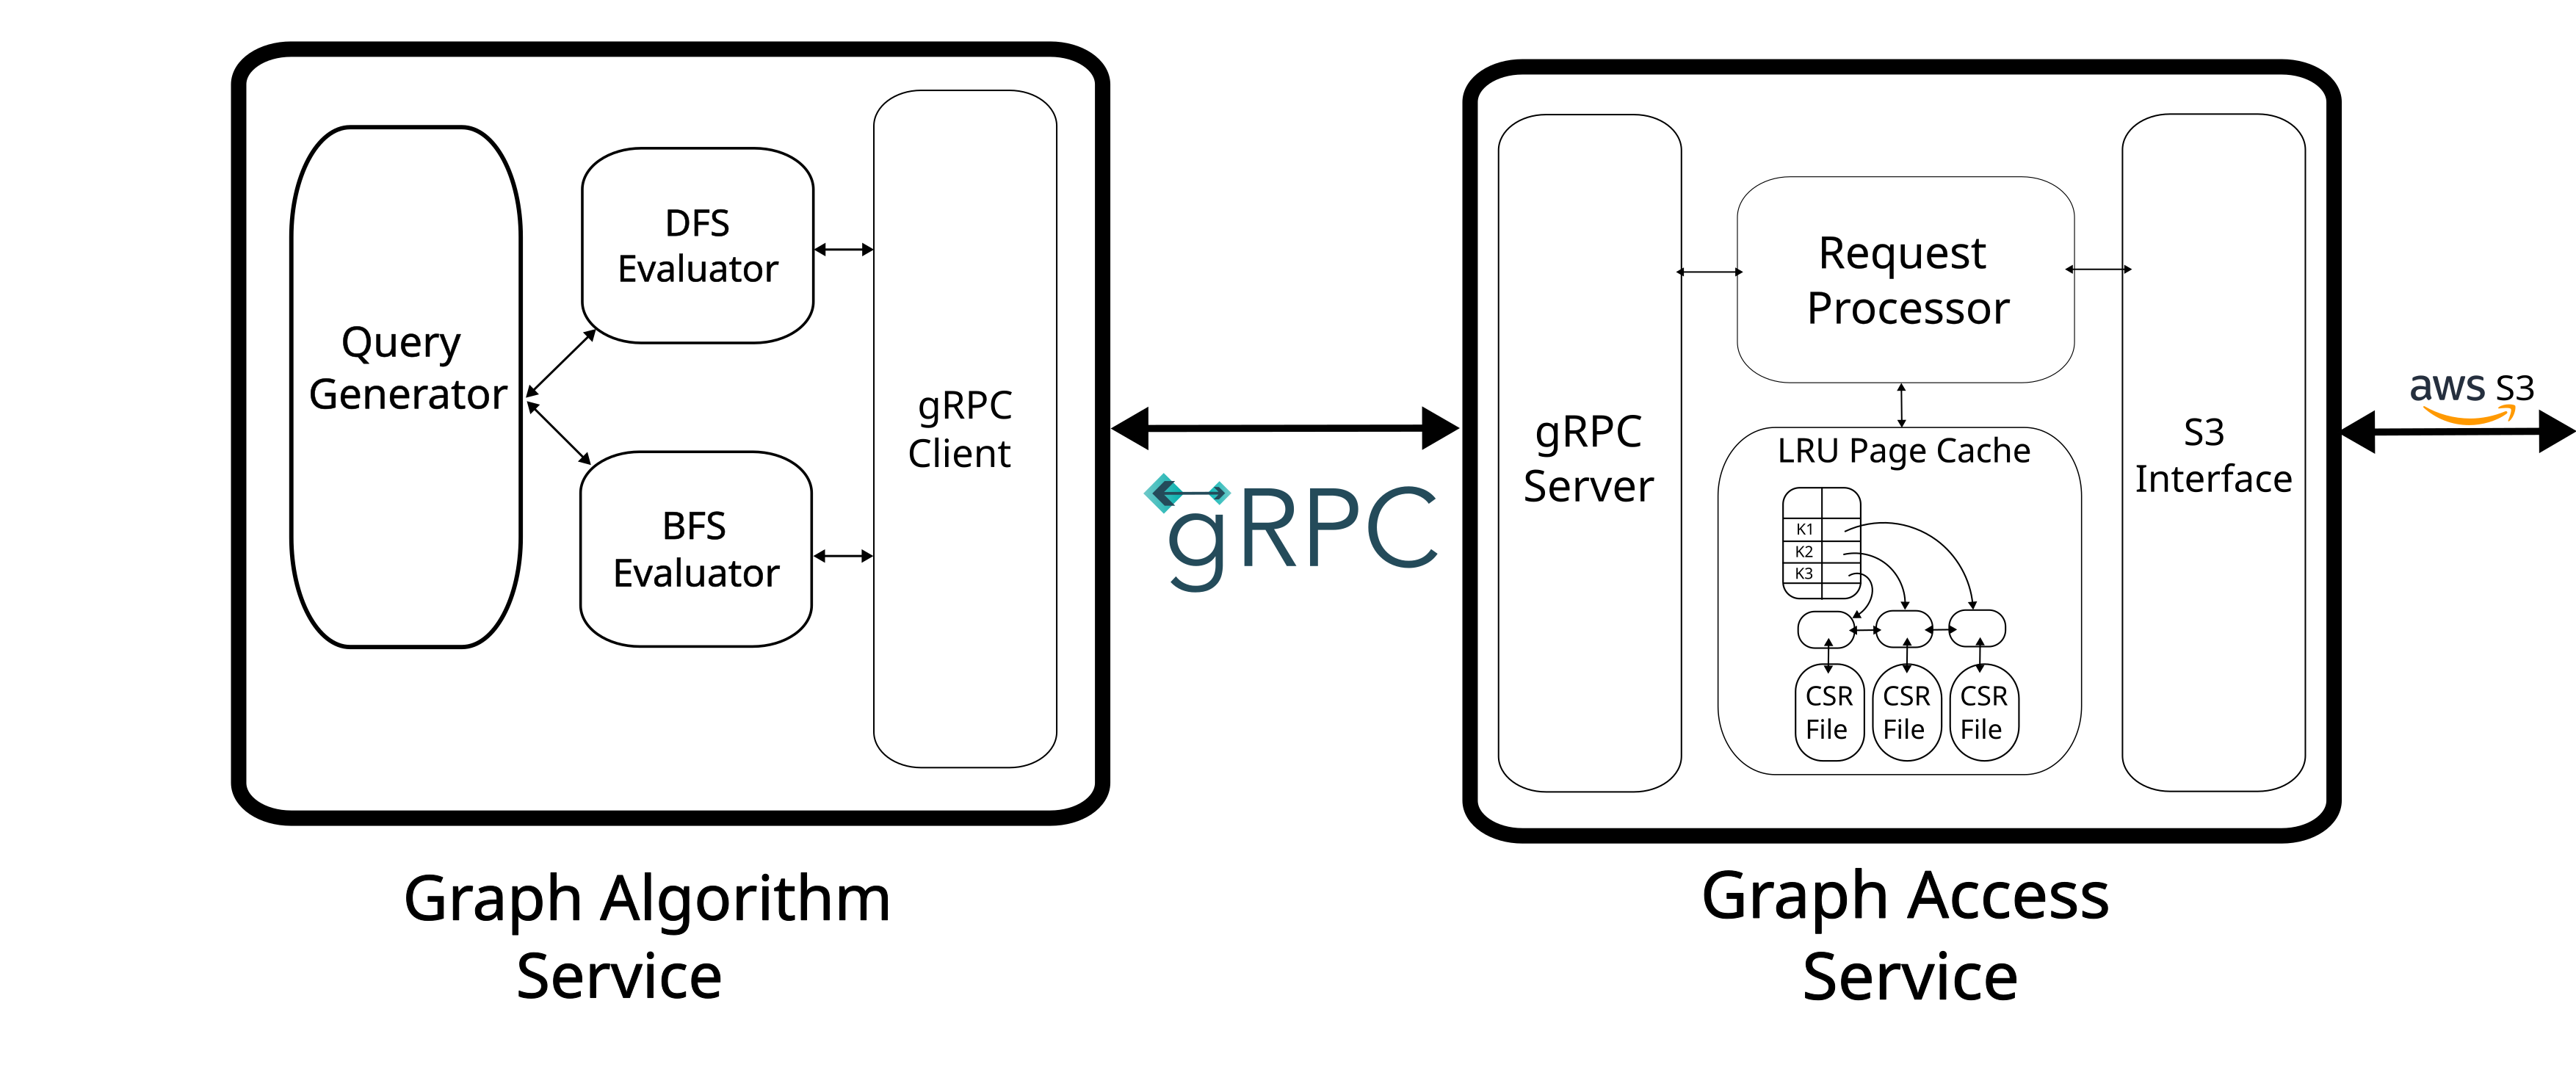
\includegraphics[width=0.8\textwidth]{figures/baseline.png}
    \caption{Baseline Implementation}
    \label{fig:baselineImpl}
\end{figure}

\medskip
The approach described in this section is quite straightforward but there are
various improvements that can be done to improve the performance and to better 
leverage the features provided by AWS S3. In the next few sections, we will
discuss how we can improve the implementation for both the graph access service
as well as the graph algorithm service. 

\section{Graph access service}\label{sec:graphAccess}
In this section, we first describe a modification of the CSR format in
Section \ref{sec:modifiedCsr} which will help us improve our cache performance.
In Section \ref{sec:accessCachePrefetching}, we describe how we leverage
this updated file format and employ the caching schemes mentioned in
Section \ref{sec:cachingDistSys}.

\subsection{Modified CSR structure}\label{sec:modifiedCsr}
In the baseline implementation of graph access service described in
Section \ref{sec:baseline}, we had to download entire files to access
a node's neighbours. This approach suffers from a couple of problems, which makes
fetching inefficient and restrictive. The first problem is that we have to
fetch and parse the information for an entire file in order to access a single
node's neighbours which is wasteful. Furthermore, this approach hinders our
ability to achieve a  higher level of granularity for better cache performance.
Second, this approach makes it harder to utilize the fact that AWS S3 replicates
files to various servers. Due to these problems, we decided to modify the
underlying binary format and the way we fetch a node's neighbours.

\medskip
Figure \ref{fig:csrFormat} shows the binary format we use for fetching a
node's neighbour. This format can logically be divided into three layers. The
first layer, which is always of a constant size, contains the first and last
node identifier present in this file. The second layer contains the byte offset
for the first incoming edge for a node and the first outgoing edge for a node.
Since these offsets are of a constant size and the fact that the first layer of
the header indicates how many nodes are present in this file, we can calculate
the size of this second layer. The third and final layer contains the edge
information, which in our case consists of the edge label and the edge
destination. This type of structure closely resembles a traditional CSR format
except for the fact that we store both incoming and outgoing edges in the same
array and that we store byte offsets instead of array indices.
\begin{figure}[ht]
    \centering
    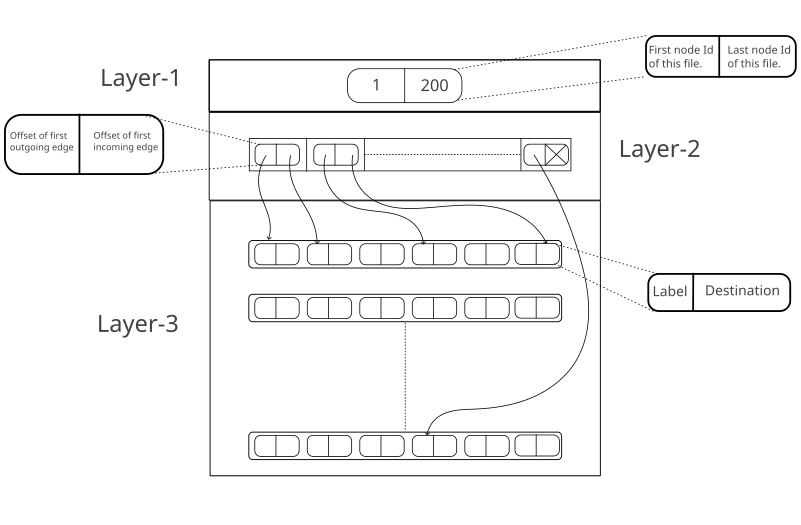
\includegraphics[width=0.8\textwidth]{figures/csrFormat.png}
    \caption{Updated CSR Format}
    \label{fig:csrFormat}
\end{figure}

\medskip
The aforementioned format gives us the ability to fetch a node's neighbours
without having to download an entire file. With this modified structure, we can
store the first layer of every file in memory and fetch the second layer of a
file when it is first accessed. After doing so, we would be able to fetch a
node's incoming or outgoing neighbours without any additional overhead.
Furthermore, we can now parallelize requests to a single file, which would lead
to better throughput since these requests would likely be distributed to
different instances within AWS S3. As an additional benefit, we can now perform
caching on a more granular level since we do not incur the overhead of fetching
and parsing an entire file whenever we need to access a node's neighbours.

\subsection{Caching and Prefetching}\label{sec:accessCachePrefetching}
Figure \ref{fig:graphAccessArch} shows the final architecture of the graph
access service. The service consists of three basic parts:
\begin{enumerate}
    \item \textbf{Interfaces for external communication}: There are two 
        components which provide an interface with external resources and are
        colored grey in the figure. The first component, on the left,
        exposes a gRPC interface which receives requests for accessing a node's
        neighbours, starting traversals, and ending traversals. The second
        component, on the right, is responsible for accessing AWS S3. This component
        takes a filename along with starting and ending file offsets and returns
        the requested file content.
    \item \textbf{Orchestration}: There are two components that help with
        orchestration of request and are colored blue in the figure. The first
        component is the `Request Processor' which is responsible for
        interacting with the caches, moving data between caches, and fetching
        data from AWS S3 in case it is not present in the caches. The second
        component titled `Vertex offsets' contains metadata related to the CSR
        format that we described in Section \ref{sec:modifiedCsr}.
    \item \textbf{Caches}: There are two different types of caches that are used
        in this service and are colored green in the figure. The first of these
        components is an LRFU cache which is used to store nodes that were
        previously accessed. The second component is a per-query prefetcher
        which fetches the nodes that are likely to be accessed by a client in
        the near future. The rest of this section is devoted to the description
        of these two components.
\end{enumerate}
\begin{figure}[ht]
    \centering
    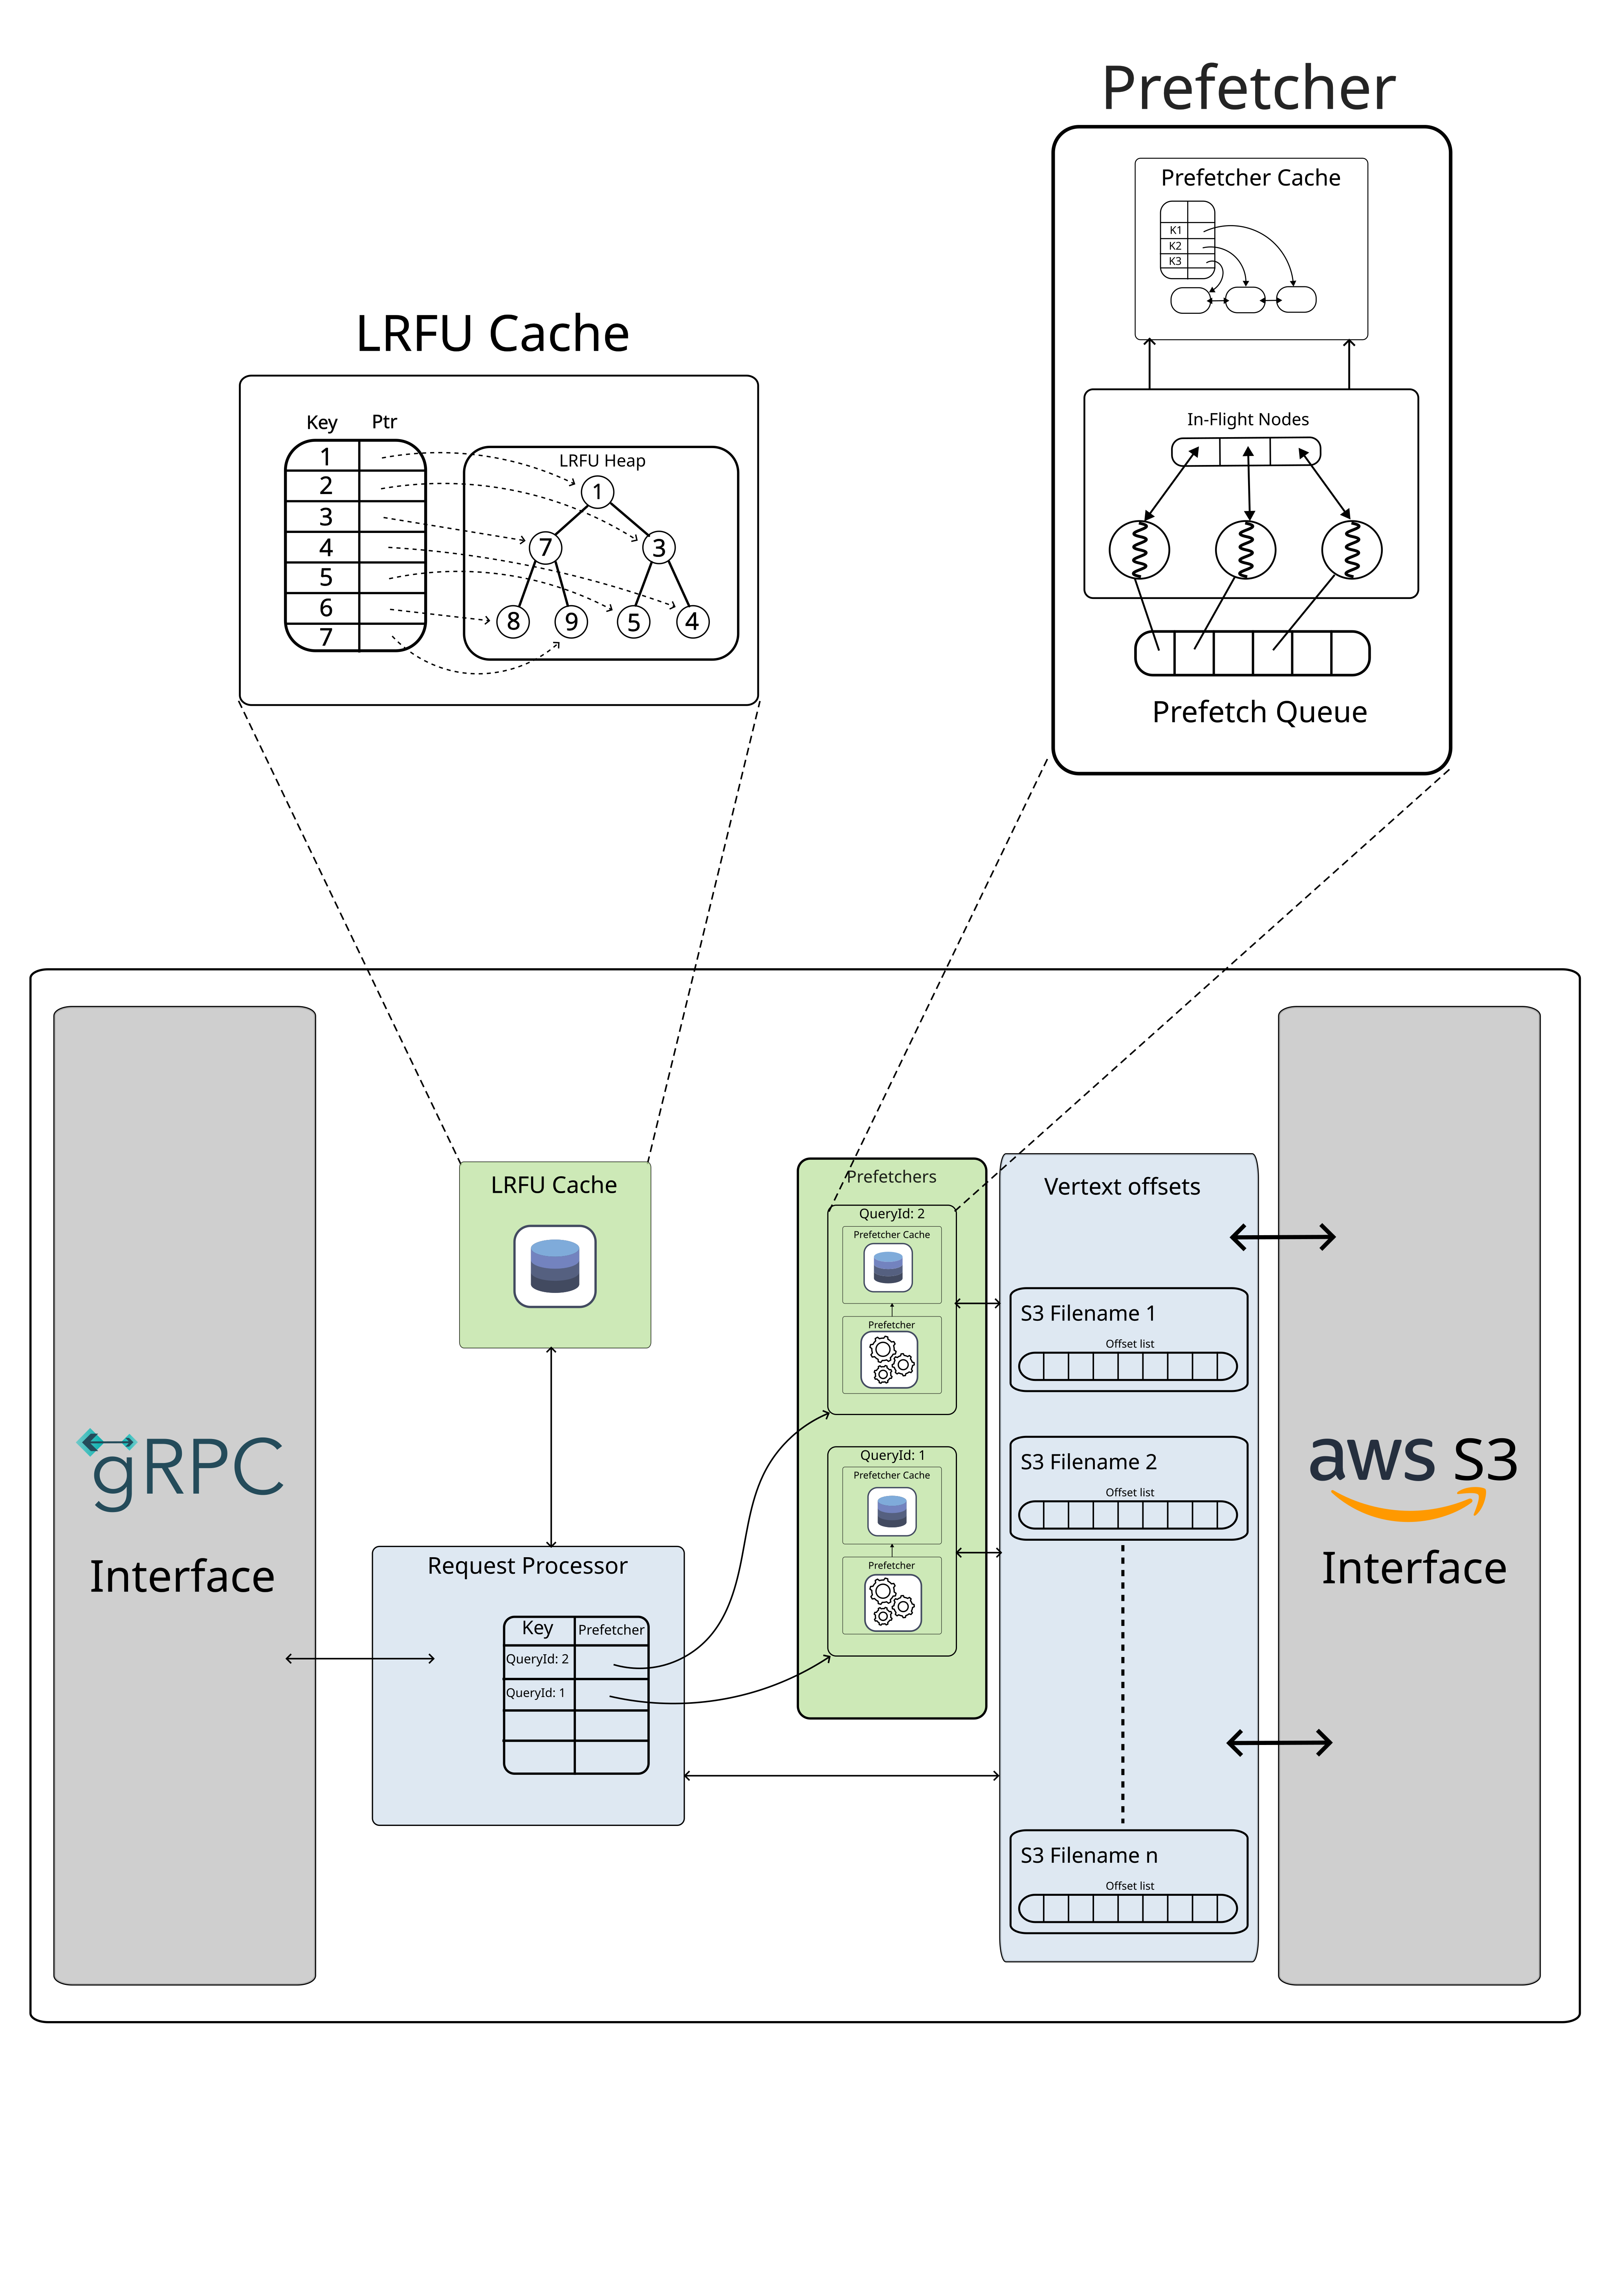
\includegraphics[width=\textwidth]{figures/graphAccessServiceFinal.png}
    \caption{Graph Access Service}
    \label{fig:graphAccessArch}
\end{figure}

\medskip
The first major component of our cache in the \textbf{LRFU
cache}\cite{lee2001lrfu}. As mentioned in Section \ref{sec:cachingDistSys}, the
main idea of this cache is to take both recency and frequency into account while
making the decision about which item to evict from the cache. While initializing
this cache, we make a decision about how much weight should be given to an
objects recency versus its frequency. Note that unlike perfect-LFU schemes, we
only store the frequency of the elements present in the cache. After
initializing the cache, it maintains a heap of elements where each element is
assigned a score based on the last time it was accessed along with its
frequency. The key to maintaining this heap is the realization that the relative
ordering of the heap remains constant if none of the elements are accessed. This
is because the degradation of score due to ageing happens at the same
rate for every element. This means that only a change in frequency can alter
the relative ordering of elements, and since the frequency only changes when an
object is accessed, we only need to change the position of the accessed node
within the heap. This enables us to perform access and insertion operations in
$\mathcal{O}(\log(n))$ time. Although simple LRU cache implementations have an
access and insertion time complexity of $\mathcal{O}(1)$,  this cache provides 
us with a good tradeoff between time complexity and flexibility for 
different workloads. We will talk more about the empirical evidence supporting
our choice in the next chapter.

\medskip
The next component, \textbf{the Prefetcher}, is inspired by the work done
by Bok et al. \cite{bok2020memory}. This component fetches the neighbours of
nodes that were accessed by a particular traversal. Every time a node's
neighbours are fetched, these neighbours are added to the `Prefetch Queue'. The
elements from this prefetch queue are read by the worker threads that are
attached to every prefetcher cache. These worker threads send our requests to
fetch the neighbours of nodes in the prefetch queue and add the nodes to the
`In-flight queue' while they wait for the response. Finally, once the neighbours
for a node are available, they are added to the prefetcher cache which is a
standard LRU cache. We will now discuss some of the design choices that we have
made for this cache.

\medskip
First, if there are multiple traversals happening, we would create a separate
prefetcher for each traversal. This choice ensures that there is minimal
interference on the performance of a traversal depending on other traversals
that may be happening. This comes with the added cost of having more worker
threads. However, using a green-thread model or asynchronous programming can help
mitigate this issue to a large extent. 

\medskip
Apart from separate prefetcher caches, we also have an `In-flight Queue' within
each prefetcher. This is useful because of the time gap between sending a
request and getting a response. This time, as we will see in the next chapter,
is an order of magnitude greater than the time scale at which the graph access
service and the graph algorithm service work. Therefore, it makes sense to have
a small amount of extra memory to ensure that if a request is already in
progress, we do not make a duplicate request, which would almost always take
longer to execute. 

\medskip
Finally, we note that the size of the prefetch queue is finite. Therefore, we
need to have some strategy to handle the case when this prefetch queue is full.
We argue that this strategy needs to be different for both BFS and DFS. This is
due to the relevance of nodes that are added to this prefetch queue. The node at
the front of the queue in BFS will be accessed earlier than the neighbours of a
node we are trying to add to the queue. However, in case of DFS, the
opposite is true because the node we are trying to add is likely the node
at the top of the stack and would be accessed next. This leads us to having two
different strategies for dealing with a full prefetcher queue for BFS and DFS:
\begin{enumerate}
    \item \textbf{BFS}: In case of BFS, the prefetcher queue behaves like a
        queue data structure and if the queue is full, the newer elements are
        discarded.
    \item \textbf{DFS}: In case of DFS, the prefetcher queue behaves like a
        stack data structure and if the queue is full, the newer elements
        are added to the top of the stack, and the elements at the bottom of the
        stack are discarded.
\end{enumerate}

\bigskip
In this section, we described a file format that enables us to perform caching
at a more granular level, and we described how this granular caching helps us
design caches that may be better suited for masking AWS S3's access latency.
In the next section, we turn our
attention to graph algorithm service where we will modify our traversals to
better fit the capabilities of AWS S3.


\section{Prallelizing traversals}\label{sec:parallelAlgorithms}
One of the main advantages of using AWS S3 is that it is able to sustain a very
high-throughput. The caching mechanisms mentioned in the previous sections
reduce the latency for accessing a node's neighbours and mitigate expensive
network calls to AWS S3 in the hot-path. These components do help with reducing
latency but they do not do anything to ensure that make use of the
high-throughput provided by AWS S3. In order to do that, we parallelize our
traversal algorithms. In this section, we will present parallel implementations
of BFS and DFS that would help us speed up our traversals by utilizing the
high-throughput of AWS S3.

\subsection{Parallel BFS}
Parallelizing breadth-first search in relatively straightforward.
Listing-\ref{lst:parallelBFS} contains the pseudo-code for our implementation of
parallel BFS. This implementation contains two queues, one for the current level
and the other for the next level of the traversal. Instead of processing the
current level within a single thread, we launch a predefined number of workers
who take elements from the queue at the current level in a work stealing
fashion and add their results to the next level of the traversal. The addition
of nodes to the next level as well as to the set of seen nodes needs to be
synchronized in accordance with the threading model of the language of
implementation.
\begin{lstlisting}[caption={Parallel BFS}, label={lst:parallelBFS}, captionpos=b, language=Python]
def ParallelBFS(startNode: nodeId, edgesToFollow: list[Edge]) -> list[nodeId] {
    startQueue = Queue[nodeId](startNode)
    for edge in edgesToFollow {
        nextLevelQueue = Queue[nodeId]()
        seen = Set[nodeId]()
        for i = 0; i < MAX_WORKERS; i++ {
            ## Use language provided utility to launch BFSWorker.
            launch_worker(startQueue, nextLevelQueue, seen, edge)
        }
        await_completion()

        startQueue = nextLevelQueue
    }

    return startQueue
}

## Operations on input, output, and seen are synchronized between
## workers. 
def BFSWorker(input, output: Queue[nodeId], seen: Set[nodeId], edge: Edge) {
    while (input.hasMoreElements()) {
        toProcess = input.Poll()
        neighbours = fetchNeighbours(toProcess, edge)
        for neighbour in neighbours {
            if neighbour not in seen {
                seen.add(neighbour)
                output.add(neighbour)
            }
        }
    }
}
\end{lstlisting}
Figure \ref{fig:parallelBFS} contains an example of how this algorithm would
work for a simple tree like graph shown on the left side of the figure. The
figure also contains three workers that are colored green, blue, and red.
This figure shows three iterations of the algorithm, along with how the
distribution of work might take place. We now describe each of these three
iterations:
\begin{enumerate}
    \item \textbf{Iteration 1}: In the first iteration, where we only have a
        single node, this node gets assigned to one of the workers at
        random. In this case it gets assigned to the green worker. At this
        stage, the green worker fetches the neighbours of this node and adds
        them to a shared set, which will be used as the starting point for the
        next iteration. In this case, the worker adds nodes 2,3,4, and 5 to this
        shared set.
    \item \textbf{Iteration 2}: In this iteration, the nodes from the shared set
        of the previous iteration are distributed among all three workers. Just
        like the previous iteration, every worker fetches the neighbours of the
        nodes assigned to them and adds the result to a shared set. In this
        iteration, nodes 2 and 3, which are assigned to different workers, try
        to add the node 7. This is the reason why we need a shared set,
        otherwise, we may end up processing node 7 twice in the next iteration.
    \item \textbf{Iteration 3}: Just like the previous iteration, the nodes from
        the shared set are distributed across workers. Subsequently, these
        workers add the neighbouring nodes of their assigned nodes to the shared
        set.
\end{enumerate}
\begin{figure}[ht]
    \centering
    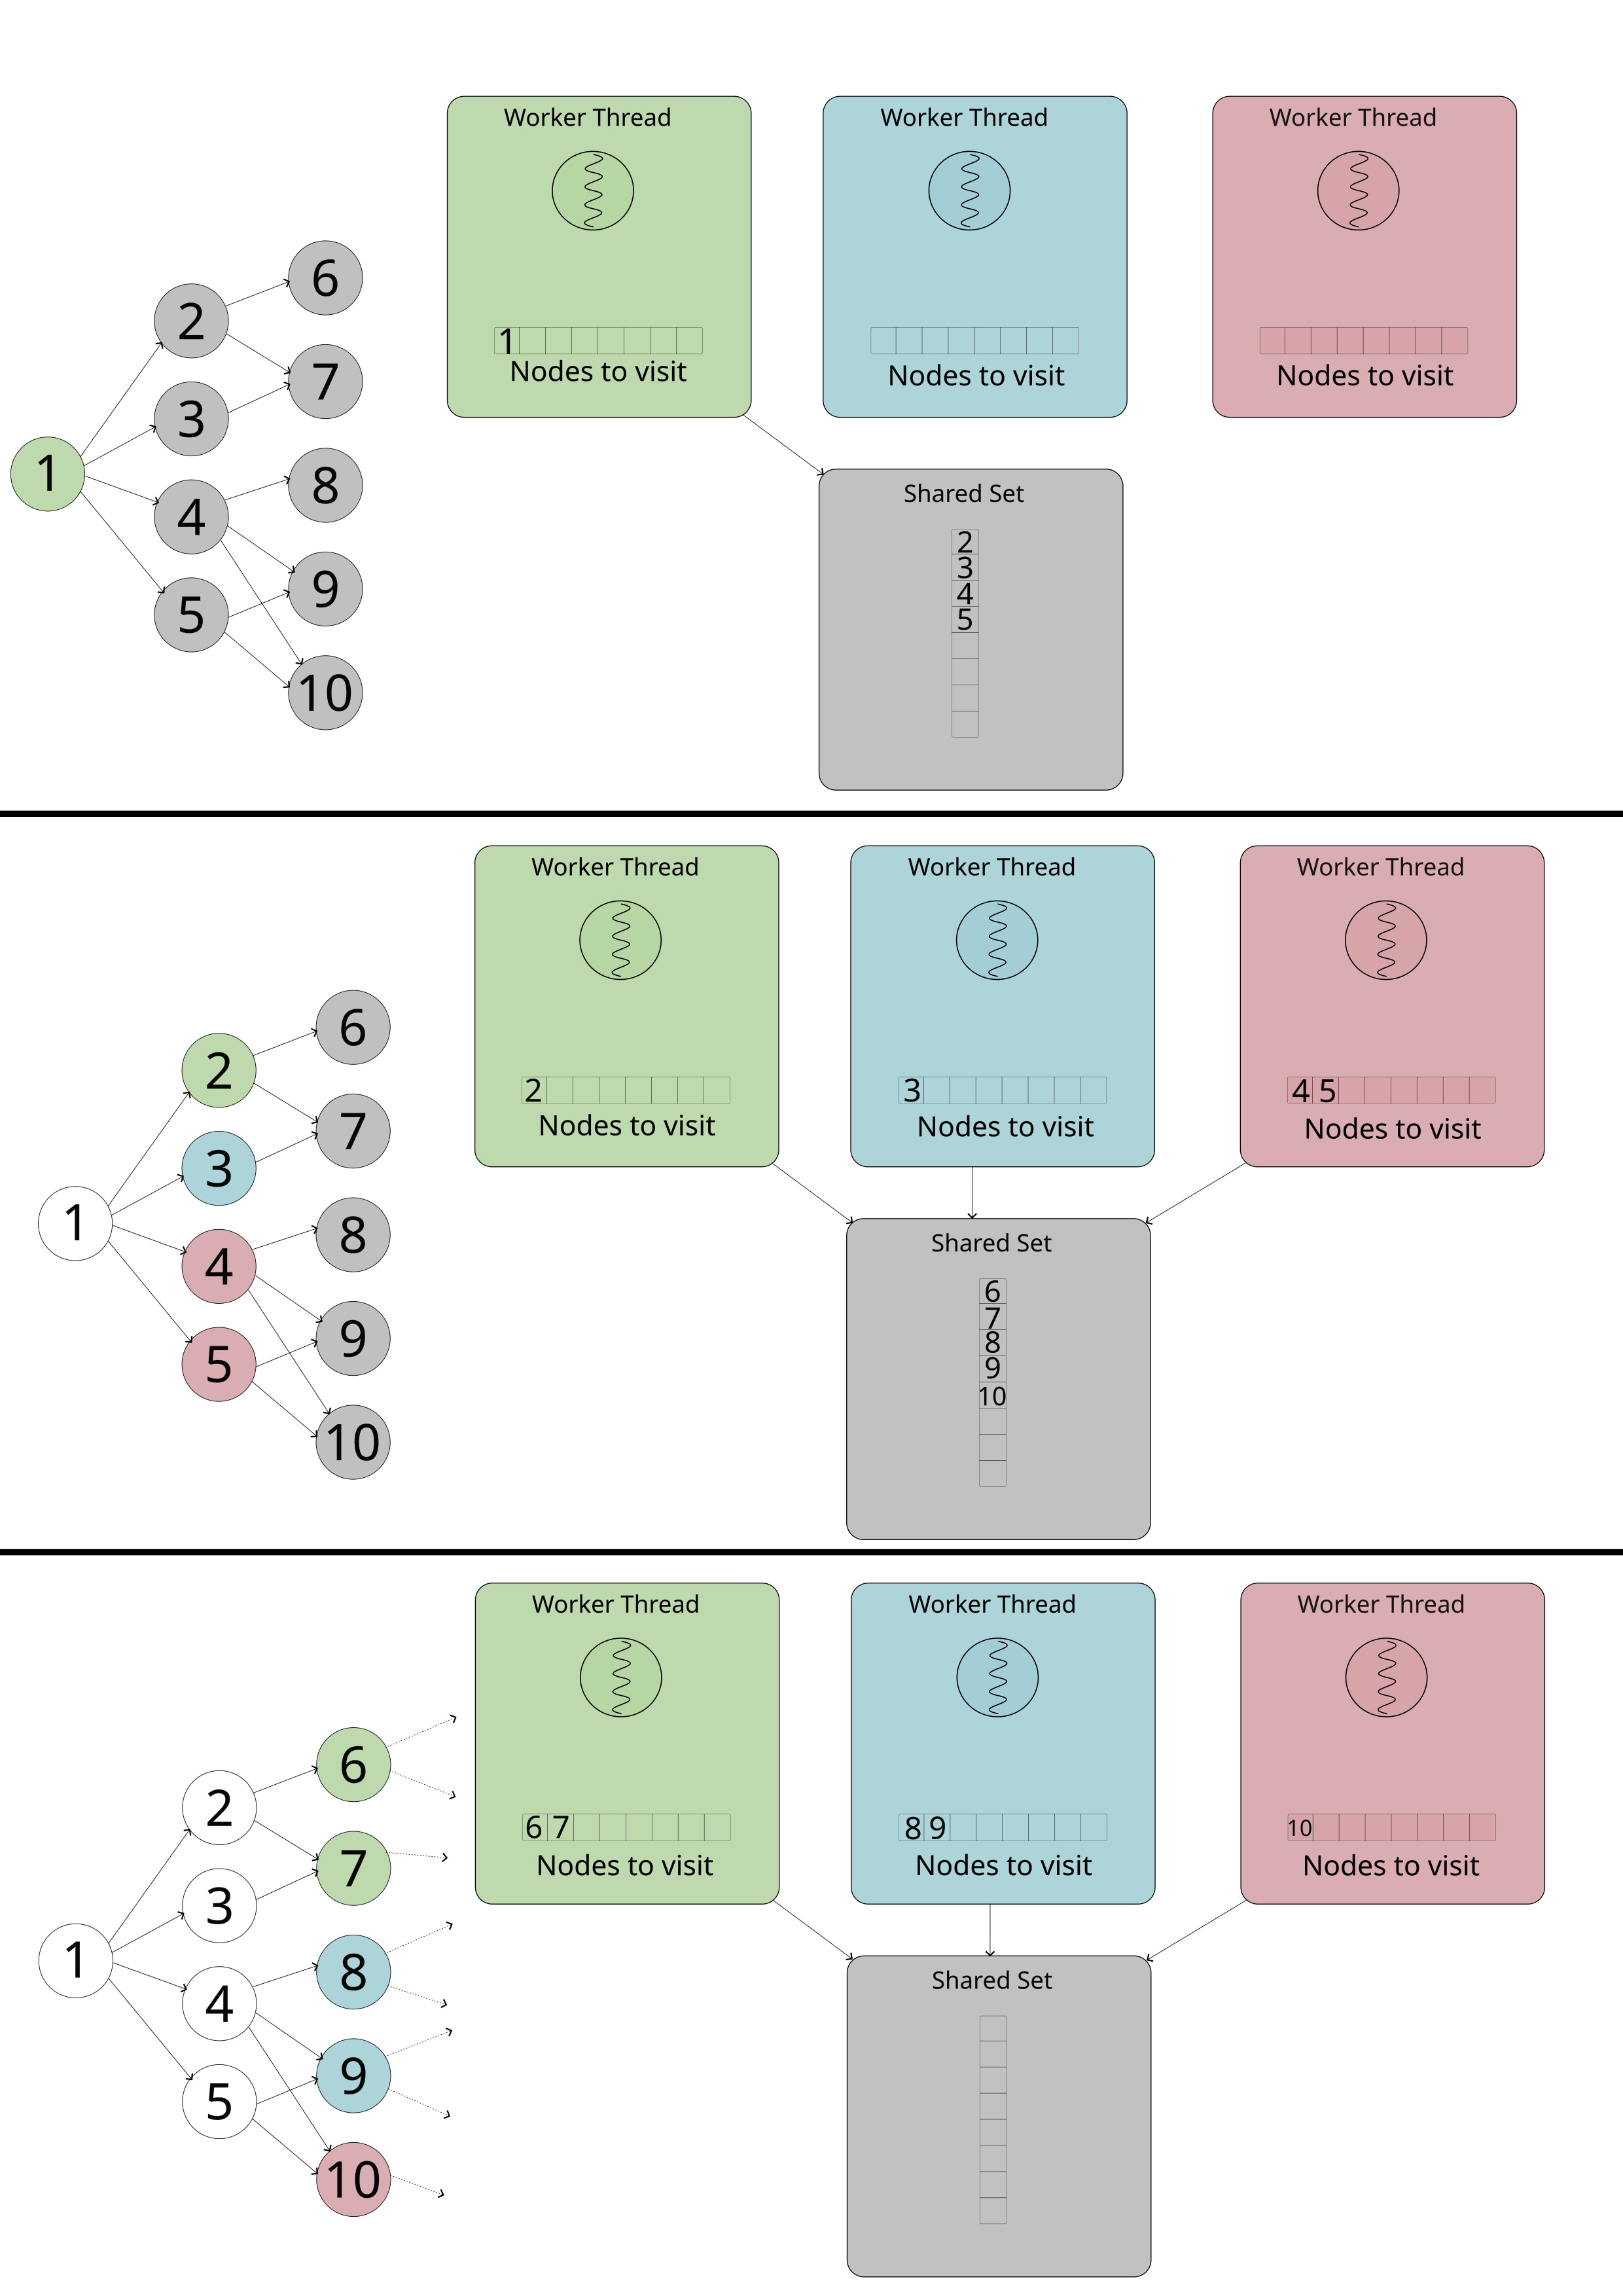
\includegraphics[width=0.75\textwidth]{figures/parallelBFS.png}
    \caption{Parallel BFS}
    \label{fig:parallelBFS}
\end{figure}

\subsection{Parallel DFS}
In this section, we describe our approach for parallelizing depth-first search.
Before we begin our description, it is important to note why a strategy similar
to the one described in the previous section would not result in equal
allocation of work. If we simply delegate the task on performing DFS on a node's
neighbours to different worker threads, then it is possible that some worker
threads might terminate significantly earlier than others. This is because the
number of nodes that can be explored from a given node might vary significantly
from one node to the other. Let us take the example of traversing a social
network graph where we start with a single person and find people connected to
this person till a certain depth. If the starting person has two friends `A' and
`B', let us assume that `A' has no friends while `B' is a celebrity and has many
friends. In this case, if we assign the work of perfroming DFS from `A' to one
worker and the work of performing DFS from `B' to another worker, we would end
up with an uneven distribution of work. This is because performing DFS on `A'
would require no further processing while the DFS on `B' is likely to go on for
quite a few iterations. Due to this problem, we need a better way to parallelize
depth-first search.

\medskip
The main idea of our approach is to dynamically rebalance the amount of work
being done by each worker in every iteration. One way to perform this dynamic
rebalancing was suggested by Rao et al.\cite{rao1987parallel} where they suggest
a work stealing algorithm in which a worker `steals' nodes from other workers'
stacks when its own stack becomes empty. Our algorithm, as shown in 
Listing-\ref{lst:parallelDFS} works on a similar principle. The one notable
difference is that instead of stealing work, every worker proactively assigns
work to different workers after fetching a node's neighbours which ensures that
the difference between the amount of work is minimized. Another important point
to note about the implementation is the structure of the data structure that
stores seen nodes. Instead of simply storing nodeIds, we store nodeId along with
the level at which a node was seen. This is done to ensure that for a traversal
with max depth `d', we return all the nodes that can be reached by taking `d'
steps from the source node.
\begin{lstlisting}[caption={Parallel DFS}, label={lst:parallelDFS}, captionpos=b, language=Python]
def ParallelDFS(startNode: nodeId, edgesToFollow: list[Edge]) -> list[nodeId] {
    stack = Stack[nodeId, level]((startNode, 0))
    seen = Set[nodeId, level]()
    result = Collection[nodeId]

    while stack.isNotEmpty() {
        toProcess := stack.pop()
        ## Termination condition
        if toProcess.level == edgesToFollow.size() {
            result.add(toProcess.nodeId)
            continue
        }
        ## Fetch the neighbours according to the edge that should be followed at
        ## this level.
        nextLevel = toProcess.level+1
        neighbours = fetchNeighbours(toProcess.nodeId, edgesToFollow[toProcess.level])
        neighbours = filterSeen(neighbours, seen, nextlevel)

        numWorkersAvailable = getAvailableWorkers()
        ## Equally partition the neighbours into 'numWorkersAvailable+1' lists
        neighbour_partitions = divide_work(neighbours, numWorkersAvailable)

        for i = 0; i < numWorkersAvailable; i++ {
            launch_worker(neighbour_partitions[i], seen, result)
        }
    }
    await_completion()

    return result
}

## Filter out nodes that we have seen at a particular level.
def filterSeen(nodes: list[nodeId], seen: Set[nodeId, level], level: level) -> list[nodeId] {
    res = list[nodeId]()
    for node in nodes {
        if (node, level) not in seen {
            seen.add((node,level))
            res.add((node,level))
        }
    }
    return res
}

## This function mimics the original implementation with the only change being
## that the seen set is shared and that this method has its own stack.
def DFSWorker(nodes: list[(nodeId,level)], seen:Set[nodeId,level], res: list[nodeId]) {
    workerStack = Stack[nodeId, level](nodes)

    while stack.isNotEmpty() {
        ## Processing logic same as the parallelDFS function
    }
}
\end{lstlisting}

Figure \ref{fig:parallelDFS} shows an example of how this implementation works.
In this figure, we only have
two worker threads, colored green and blue. We now describe the three iterations
shown in the figure:
\begin{enumerate}
    \item \textbf{Iteration 1}: In the first iteration, the green worker thread
        processes the node 1. Before the start of this
        algorithm, the tuple $(1,0)$ is added to the shared node-level
        set. This indicates that node 1 was seen at level 0. After
        fetching the neighbours of the first node, we check if there are any
        worker threads available to take over the work for some nodes. We find
        that the blue worker is indeed idle and therefore, some of the
        neighbours can be added to its local stack. Here we assume that out of
        the three nodes, two are added to the stack of the green worker and one
        is added to the stack of the blue worker. During this partitioning, we
        also add the newly visited nodes to the shared set. 
    \item \textbf{Iteration 2}: In the second iteration, the green worker
        explores the neighbours of node 2 and the blue worker
        explores the neighbours of node 4. After exploring the
        neighbouring nodes, both of the workers check if some of the newly
        explored nodes can be added to another worker's stack. However, since
        both workers are busy, all the nodes are added to their own stacks.
        Finally, like in previous iteration, the newly visited nodes are added
        to the shared set. Notice that there is a race condition between the
        green worker and the blue worker to add node 7. In order to ensure that
        this node is not processed twice at the same level, the workers need to
        check if node 7 has been visited at depth of 2. If it has not been
        visited, then the worker will add that to the shared set and then add it
        to its stack. With this mechanism, only one of the two workers will be
        able to take responsibility for processing this node.
    \item \textbf{Iteration 3}: During the final iteration, the green worker
        will process node 5 and the blue worker will process node 7. All the
        nodes that have already been seen are also added to the shared set.
        After this stage, the two workers will go on to process nodes 9 and 10.
        Finally, the green worker will process node 3 but since all its
        neighbours have already been processed, the algorithm will terminate.
\end{enumerate}
\begin{figure}[ht]
    \centering
    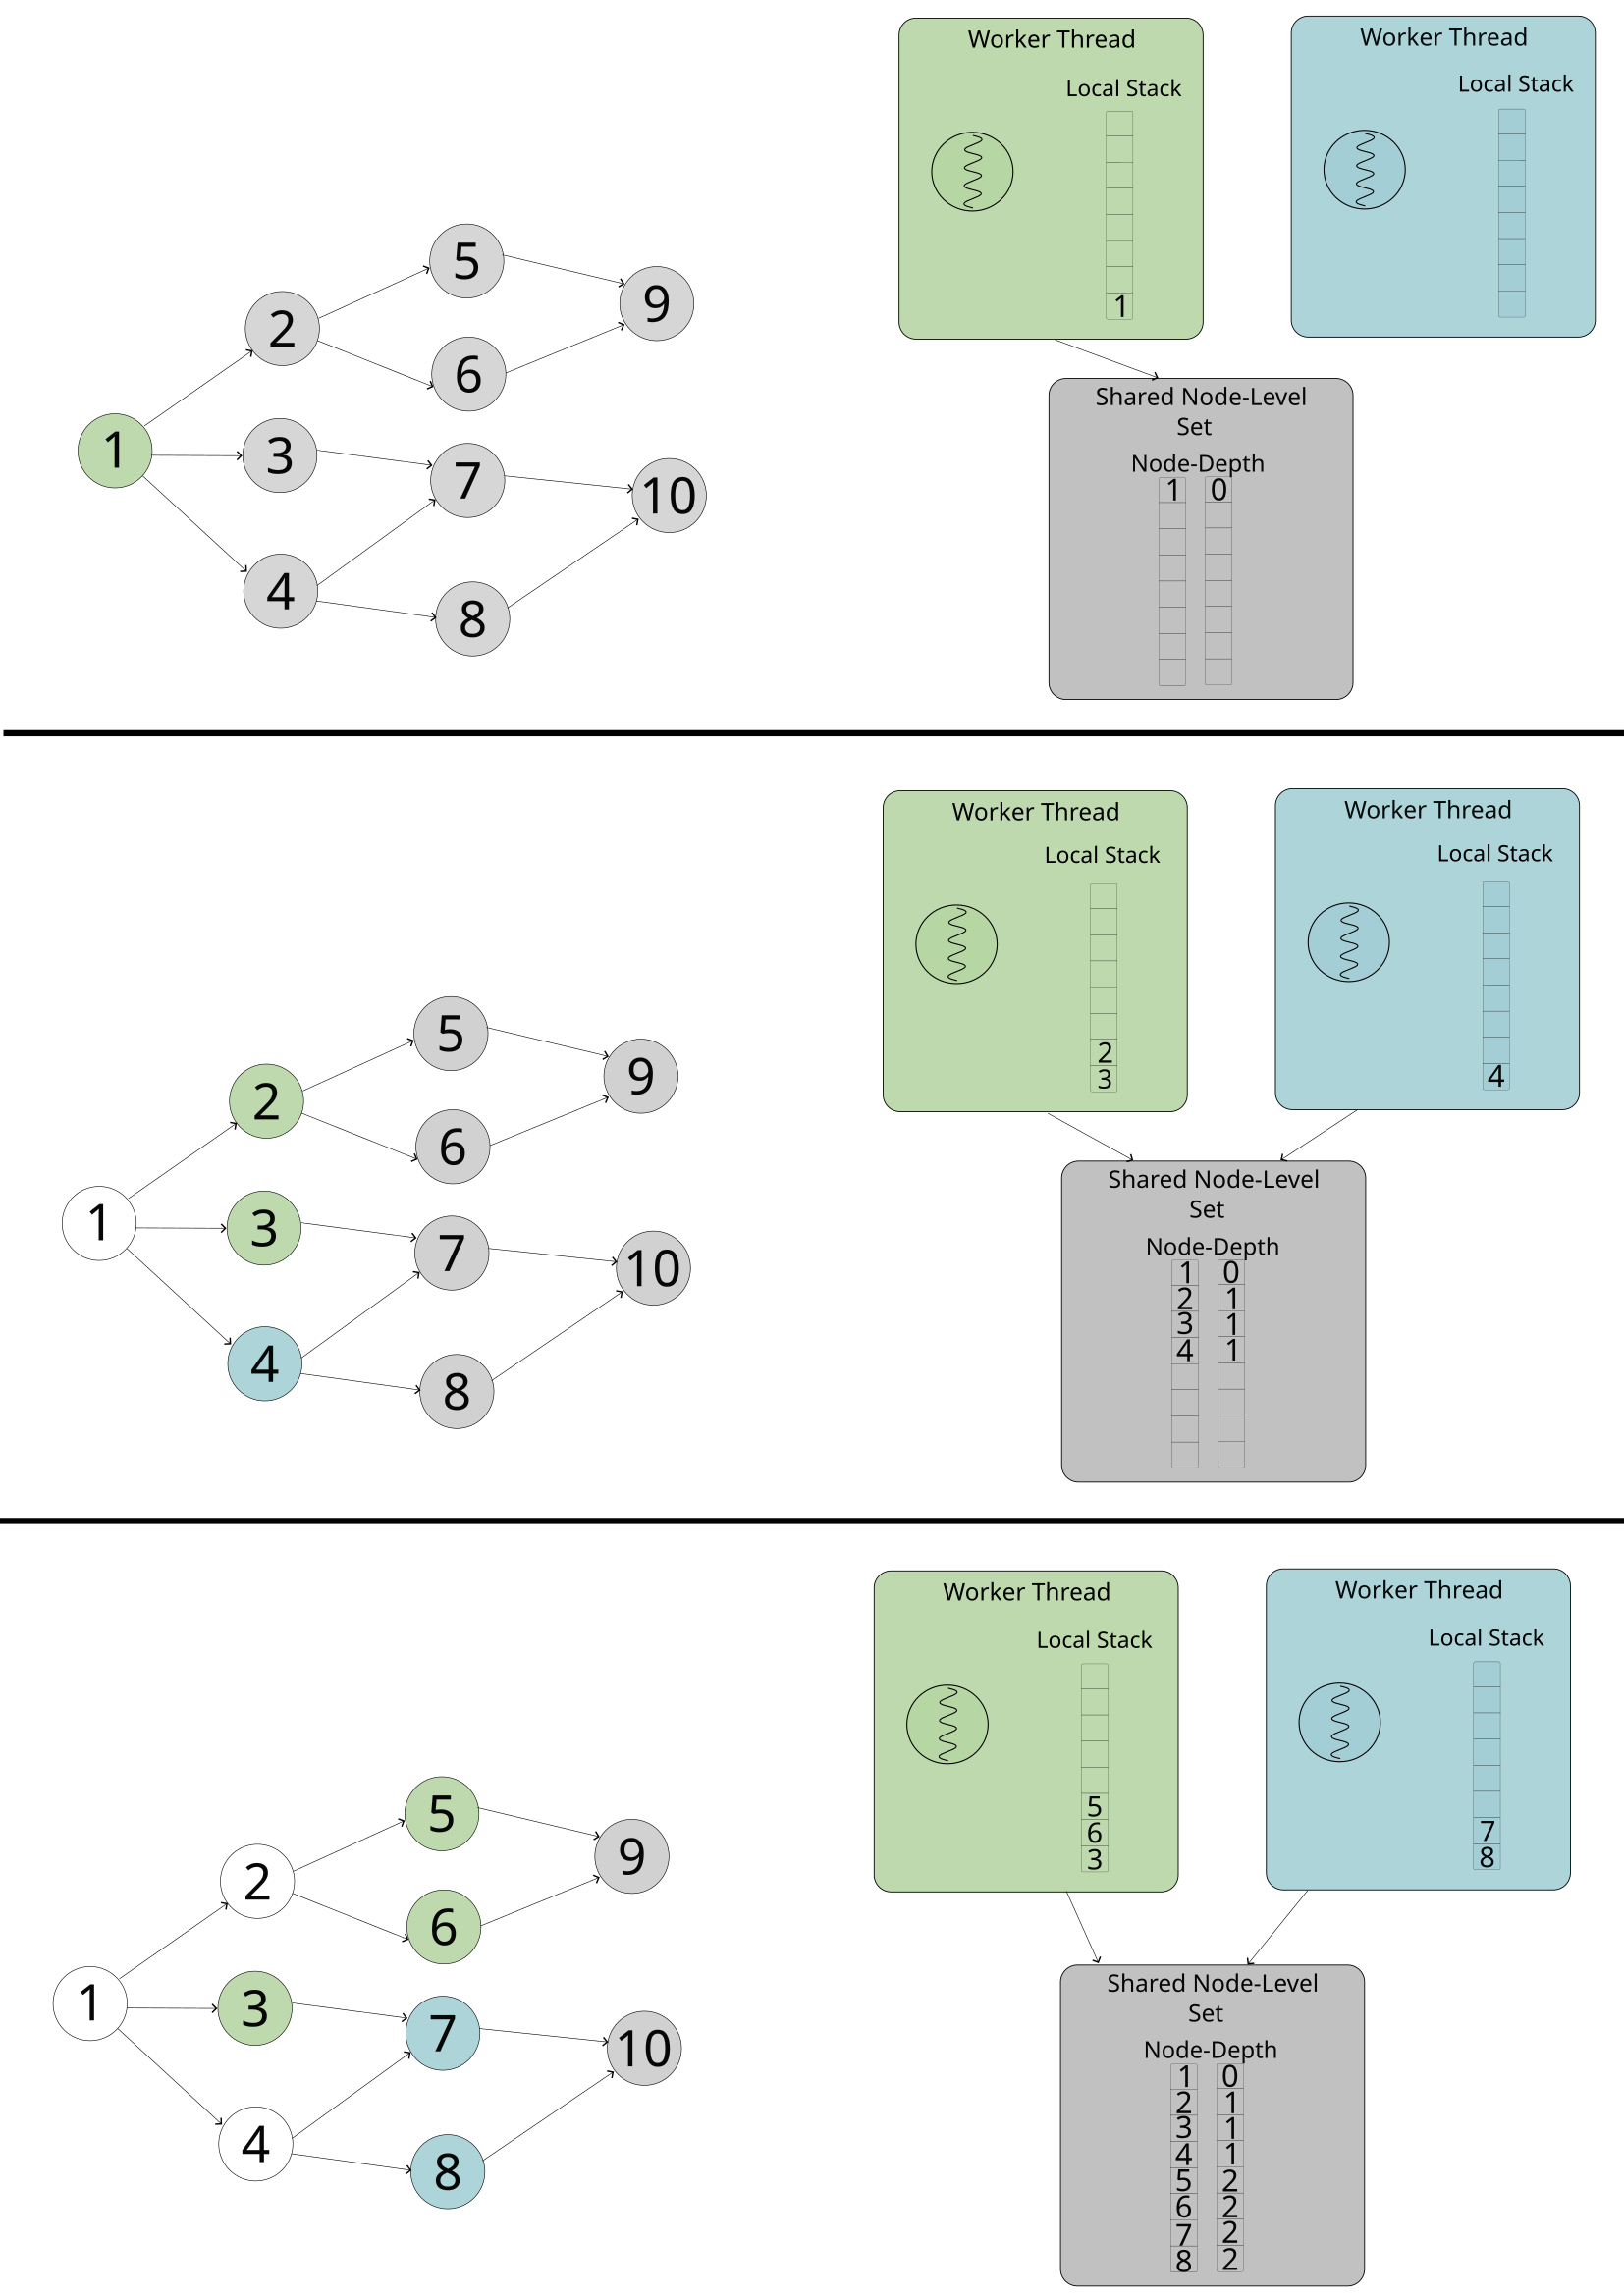
\includegraphics[width=0.75\textwidth]{figures/parallelDFS.png}
    \caption{Parallel DFS}
    \label{fig:parallelDFS}
\end{figure}


\clearemptydoublepage

\chapter{Evaluation}\label{chapter:evaluation}
Before presenting the results of our comparison with the baseline, we will
describe our benchmarking procedure. Within the benchmarking methodology, we
highlight the queries we run along with the dataset on which we run the
queries. Finally, we describe how the services are deployed and how the results
are collected.

\smallskip
Our benchmark contains a total of seven different types of queries. Each of
these seven queries starts with a random source vertex and performs the desired
traversal according to the traversal specification. A traversal specification
specifies the label and direction that needs to be followed for every hop. For
example, a traversal specification might instruct the algorithm to start from a
node of type `Person', traverse the outgoing edges with the label
`PersonKnows', and then find all the incoming edges for `PostCreator'. As a
result of running this traversal, we would get the identifiers for all the posts
created by a person's friends. The schema containing the specification of the
nodes and labels mentioned here can be found in Appendix \ref{sec:schema}. This
schema describes a social network consisting of people who can create posts
within forums, comment on posts, etc. 

\smallskip
The seven traversals that we have chosen can be divided into four parts. The
first two traversals are 1-Hop traversals, which means they only access a node's
immediate neighbours. Similarly, we have two queries for 2-Hop traversals, and
3-Hop traversals. One of the two queries in each category is chosen in such a
manner that the result cardinality is close to one, and the other query has a
higher cardinality. However, for 4-Hop traversals, the baseline implementation
was so slow that we do not have a high cardinality traversal for 4-Hops. The
following list contains the details of the queries that were used for the
evaluation. Each of these queries was repeated 20 times with different source
nodes chosen at random.
\begin{enumerate}
    \item \textbf{1 Hop}
        \begin{enumerate}
            \item \textbf{Q-1}: Start with a node of type `Forum', and traverse outgoing
                edges with the label `ForumMember'. This gives us all the forum members for
                a particular forum.
            \item \textbf{Q-2}: Start with a node of type `Post', and traverse outgoing
                edges with the label `PostContainerForum'. This gives us the container forum
                for a post.
        \end{enumerate}
    \item \textbf{2 Hop}
        \begin{enumerate}
            \item \textbf{Q-3}: Start with a node of type `Person', and traverse
                the edges with the label `PersonKnows' twice. This gives us all the
                people that a person's friends know.
            \item \textbf{Q-4}: Start with a node of type `Person', and traverse
                the edge with the label `PersonWorksAt'. After this traverse the
                relation `OrgLocation'. This gives us the locations of the
                companies that a person has worked for.
        \end{enumerate}
    \item \textbf{3 Hop}
        \begin{enumerate}
            \item \textbf{Q-5}: Start with a node of type `Person', and traverse
                the edges with the label `PersonKnows'. After this, traverse the
                edge with the label `PersonInterestTag' to get the interests of all
                these people. Finally, traverse edges with the label `TagClass' to
                find the tags for each of these interests. This query gives us
                the tags for the interests of a person's friends.
            \item \textbf{Q-6}: Start with a node of type `Post', and traverse
                the edge with the label `PostContainerForum' to get the forum which
                the post is a part of. Then we traverse the `ForumTag' label
                followed by the `TagClass' label. This gives us the tag classes for
                a post's forum.
        \end{enumerate}
    \item \textbf{4 Hop}
        \begin{enumerate}
            \item \textbf{Q-7}: This query starts with a `Comment', and looks for
                this comment's creator by following the `CommentCreator' label.
                Then, we look at the tag superclasses of this person's interest
                tag by following `PersonInterestTag', `TagClass', and
                `TagClassSuperclass' labels.
        \end{enumerate}
\end{enumerate}

\medskip
As mentioned in the previous paragraph, we run these queries on the LDBC-SNB dataset
whose schema is provided in Appendix \ref{sec:schema}. However, LDBC provides
multiple datasets with the given schema, all of which are of varying sizes.
For this thesis, we use datasets with a scaling factor of 1 and 10 (SF-1 and
SF-10). As mentioned in Section \ref{sec:componentOverview}, we convert these
datasets to a binary format before processing. During this processing, we remove
edge and node-related information since that is not needed during the traversal.
After removing the unnecessary information, we partition the adjacency into
multiple files, each of which is then uploaded to S3.
Table \ref{table:dataSpecs} contains the specifications of the two datasets that
we use.


\begin{table}[h!]
 \centering
 \begin{tabular}{|c | c | c |} 
 \hline
  & SF-1 & SF-10 \\ [0.5ex] 
 \hline\hline
     \textbf{Nodes} & 3 Million & 30 Million \\ 
     \textbf{Bidirectional edges} & 17 Million & 170 Million \\
     \textbf{Number of partitions} & 37 & 173 \\
     \textbf{Total size} & 286 MB & 2.8 GB \\
 \hline
 \end{tabular}
 \caption{Dataset specifications}
 \label{table:dataSpecs}
\end{table}

\medskip
In order to run these queries, we run the graph access service and graph
algorithm service on an EC2 instances\cite{awsEC2}. AWS provides a variety of
compute instances for different workloads. In our case, we need a general
purpose compute instance which has high bandwidth. At the time of writing this
thesis, instances labeled `c7gn' fit these specifications the best. The
particular instance that we use for most of our benchmarks is labeled
`c7gn.xlarge' which provies a network bandwidth of 50 Gbps, has 8 Gigabytes of
RAM, has 4 vCPUs, and costs 0.25 \$/hour.

\section{Comparison with baseline}\label{sec:cmpBaseline}
\begin{figure}[ht]
    \centering
    \begin{subfigure}[b]{0.48\textwidth}
        \centering
        \includegraphics[width=\textwidth]{figures/charts/BFS_cmp_1}
        \caption{BFS SF-1}
        \label{fig:bfsSf1}
    \end{subfigure}
    \hfill
    \begin{subfigure}[b]{0.48\textwidth}
        \includegraphics[width=\textwidth]{figures/charts/BFS_cmp_10}
        \caption{BFS SF-10}
        \label{fig:bfsSf10}
    \end{subfigure}
    \begin{subfigure}[b]{0.48\textwidth}
        \centering
        \includegraphics[width=\textwidth]{figures/charts/DFS_cmp_1}
        \caption{DFS SF-1}
        \label{fig:dfsSf1}
    \end{subfigure}
    \hfill
    \begin{subfigure}[b]{0.48\textwidth}
        \includegraphics[width=\textwidth]{figures/charts/DFS_cmp_10}
        \caption{DFS SF-10}
        \label{fig:dfsSf10}
    \end{subfigure}
    \caption{Baseline comparison}
    \label{fig:baselineCmp}
\end{figure}
Figure-\ref{fig:baselineCmp} contains the comparison of our final
implemnetation, as described in Section \ref{sec:graphAccess} and Section 
\ref{sec:parallelAlgorithms}, with the baseline implementation described in
Section \ref{sec:baseline}. Figures \ref{fig:bfsSf1} and \ref{fig:bfsSf10}
compare the performance of Breadth first search for scaling factor of 1 and 10.
Similarly, Figures \ref{fig:dfsSf1} and \ref{fig:dfsSf10} do the same for Depth
first search. Note that the y-axis on these graphs is logarithmic. Looking at
these graphs, we notice the following facts:
\begin{enumerate}
    \item \textbf{No benefit for small graphs}: From figures \ref{fig:dfsSf1}
        and \ref{fig:bfsSf1}, it is clear that our proposed architecture perform
        worse than the simpler baseline implementation. This is primarily
        because the number of different files is quite small for SF-1 and
        therefore most of the files required for a traversal are loaded in the first
        few runs of that traversal. After that, all the traversals are performed
        from memory.
    \item \textbf{The proposed approach scales better}: If we compare the results of
        running DFS and BFS on SF-1 and SF-10, we notice that the running times
        for our final implementation remain relatively unchanged. However, the
        running times for the baseline implementation degrade by one to two
        orders of magnitude. Furthermore, the total time for running the entire
        workload for the baseline implementation on SF-10 with BFS was around 14
        minutes whereas the running time for our proposed implementation was
        just 24 seconds. This is a 35x improvement in the running time of the
        entire workload.
    \item \textbf{BFS $>$ DFS}: These results also show that the simpler parallel
        BFS implementation works much better than the parallel DFS
        implementation. For SF-10, the entire workload took 68 seconds while
        running DFS but took only 14 seconds while running BFS.
\end{enumerate}

\medskip
TODO argue that the prefetcher yields some benefit 

\subsection{Optimizing partition sizes}\label{sec:partitionSize}
\subsection{Distributed Deployment}\label{sec:distDeploy}
\section{Comparison with other tools}\label{sec:cmpOtherTools}
\subsection{Neo4j}
\subsubsection{Monolithic Deployment}
\subsubsection{Distributed Deployment}
\subsection{Apache Flink}



\clearemptydoublepage

% This can become the discussions section instead of comparisons.
\chapter{Discussion}\label{chapter:discussion}
\section{Cost Model}\label{sec:costModel}
\section{Threats to credibility of this work}\label{sec:threats}
\section{Alternate system architectures}\label{sec:altArchitectures}


\clearemptydoublepage

\chapter{Conclusion and Future Work}\label{chapter:conclusions}
We started the paper with two research objectives pertaining to the
applicability of a graph database that separates compute and storage. The first
objective was to gauge the applicability of employing prefetching and caching
techniques to reduce the latency of accessing data in the distirbuted data
store. The second objective was to provide a cost model which might enable users
to decide whether using AWS S3 as storage backend would be more cost-efficient.
After answering these questions, we will also mention some future research
objectives that need to be achieved to create a graph database based on AWS S3.

\medskip
In section \ref{sec:accessCachePrefetching} we defined the caching and
prefetching techniques that we use to reduce the latency for our architecture.
Then in section \ref{sec:cmpBaseline}, we compare this approach with a baseline
approach and conclude that our approach provides substantially lower latency but
only for large graphs. Then, we also break down the effectiveness of each
component of our system and evaluate their effectiveness individually. After
that, we discuss how we can increase parallelism to reduce the overall running
time for a workload. Then, in section \ref{sec:partitionSize}, we
explore the effect that partition sizes have on the total time taken to run a
workload. Finally, in section \ref{sec:distDeploy}, we use a distributed
deployment to verify that we can indeed scale the performance of our solution by
adding more compute.

\medskip
In order to provide a cost model, we first compare the performance of our tools
with other state-of-the-art technologies that can be used to perform traversals
on large graphs in section \ref{sec:cmpOtherTools}. By doing this, we find that 
the case where our solution outperforms other tools is when the size of the
graph is huge and the throughput requirements are relatively low. Then in
section \ref{sec:costModel}, we provide a mathematical model to gauge the cost
of solutions that couple storage and compute to our solution. Using some
examples, we confirm that our solution is cost effective for large graphs with
low throughput requirements. Finally, we also provide some extra benefits of
using our approach as it delegates the responsibility of replication and
consistency to AWS S3.

\section{Future Work}\label{sec:futureWork}
There are a lot of avenues for future research into the approach that we have
suggested here. These opportunities for further research can be grouped into the
following buckets:
\begin{enumerate}
    \item \textbf{Handling updates}: A graph database would more often than not
        require updates. As we mentioned in section \ref{sec:threats}, there is
        some research into how this can be handled for B-trees and this research
        needs to be extended to incorporate our storage model. There may be
        multiple ways of handling updates with multiple tradeoffs in terms of
        properties like consistency, performance, and cost.
    \item \textbf{Handling properties}: In this thesis, we did not consider node
        and edge properties. We can group these properties into two categories:
        fixed size properties, and variable size properties. For variable size
        properties, like strings, we would require a different storage
        mechanism. For fixed size properties, we would need to explore how they
        could be incorporated into the CSR format that we described and how
        would we handle schema evolution.
    \item \textbf{Caching graphs}: In this thesis, we contrasted using AWS S3
        with using an SSD for storing the graph. However, we may be able to get
        the best performance by combining the two approaches. We could
        therefore, store a large parts of subgraphs into SSD for fast retrieval
        to reduce latency while still enjoying the benefits of AWS S3. We would
        need to explore how can we choose which parts of graph to store locally
        based on workloads or graph characteristics.
\end{enumerate}


\clearemptydoublepage

%Choose a good bibliography style, plain would do often, but these might be nice too
%\bibliographystyle{these}
\bibliographystyle{plain}
\bibliography{./references}

\clearemptydoublepage

\appendix
\addcontentsline{toc}{chapter}{Appendix}

\chapter{SNB Schema} \label{sec:schema}
\begin{figure}[ht]
    \centering
    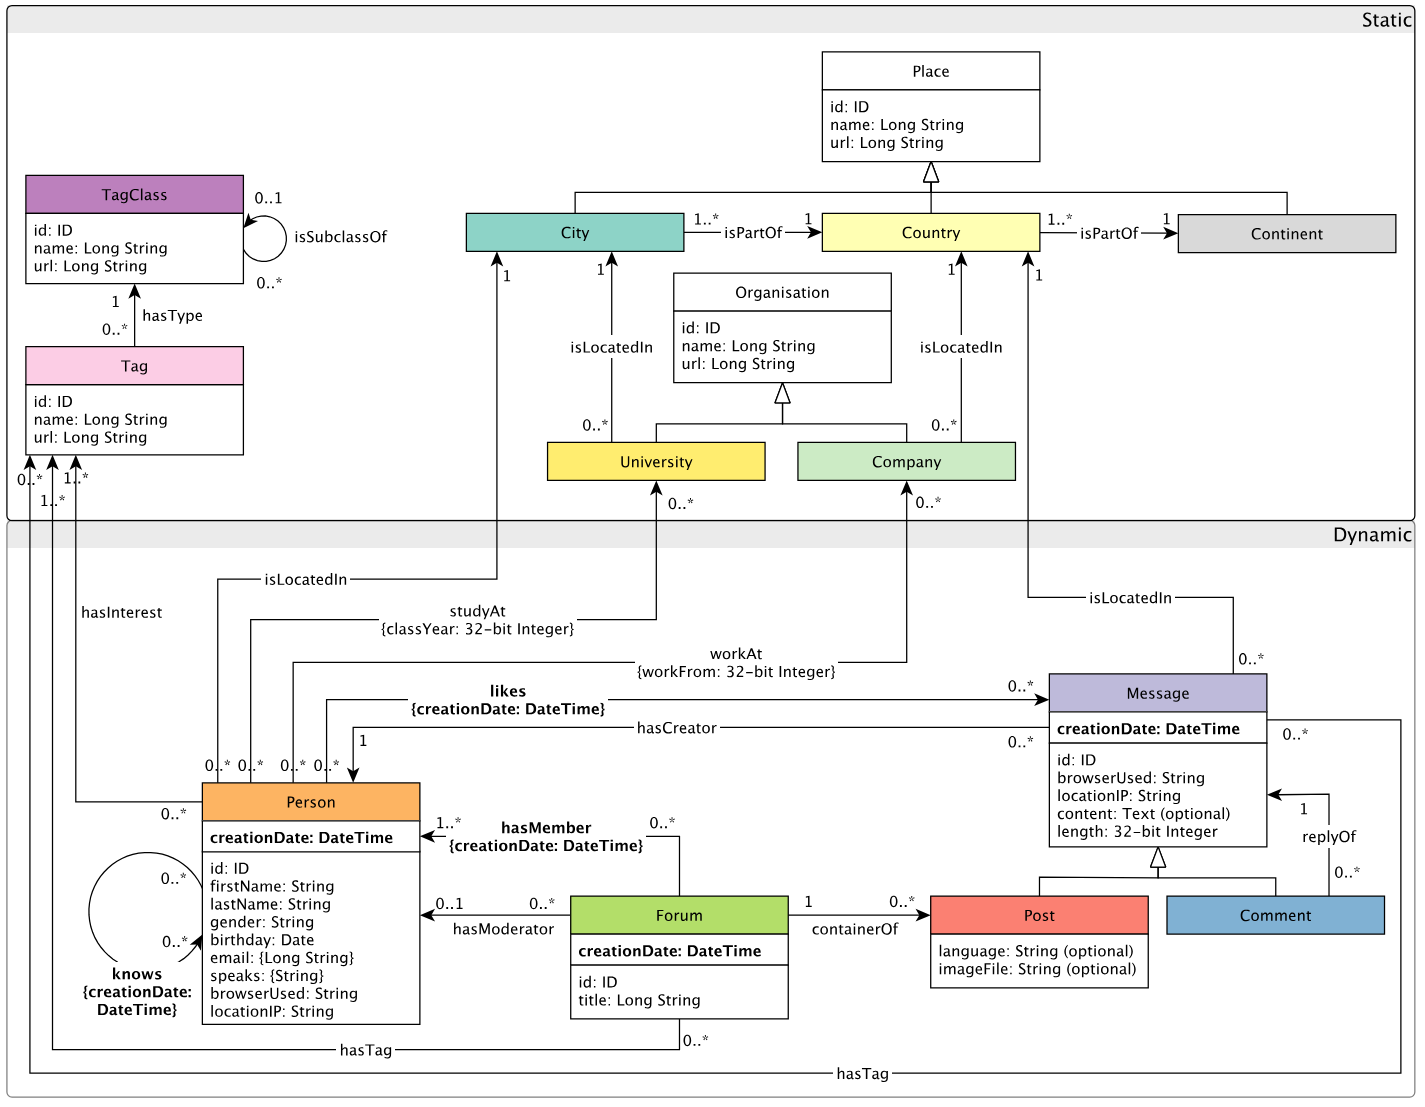
\includegraphics[width=0.9\textwidth]{figures/LDBC-Schema}
    \caption{LDBC SNB Schema}
    \label{fig:ldbcSchema}
\end{figure}
Figure \ref{fig:ldbcSchema} contains the schema of the dataset that was used in
this thesis. This schema along with the underlying dataset was generated as per
the specifications of the LDBC social network benchmark\cite{angles2020ldbc}.


\end{document}
